\documentclass{scrreprt}
\usepackage[utf8]{inputenc}
\usepackage{ngerman}
\usepackage{amsmath, amsfonts, amssymb}
\usepackage{algorithm, algpseudocode}
\usepackage{graphicx}
\usepackage[section]{placeins}
\usepackage{textgreek}
\usepackage{scrhack}

\graphicspath{{./Abbildungen/}}
\title{Analyse der Druckberechnung mithilfe einer Zustandsgleichung im Vergleich zur Lösung eines Gleichungssystems in SPH- Flüssigkeitssimulationen}
\author{Pascal Hunkler}
\date{May 2022}

\begin{document}

\maketitle

\setlength{\parindent}{0pt}
\setlength{\parskip}{1em}

\tableofcontents

\chapter{Abstract}
\chapter{Einleitung}
\chapter{Grundlagen}
\section{Navier-Stokes-Gleichung und Flüssigkeitssimulationen}
Dieser Abschnitt behandelt die Navier-Stokes-Gleichung, welche die Grundlage dafür bildet, Flüssigkeitssimulationen zu realisieren.
Sie beschreibt die Änderungsrate der Geschwindigkeit eines kleinen volumetrischen Flüssigkeitelements.
Für die Navier-Stokes-Gleichung gibt es verschiedene Formen, die auf den eulerschen Ansatz oder den lagrangeschen Ansatz beruhen.
Diese Arbeit beschäftigt sich im Wesentlichen auf lagrangesche, partikelbasierte Simulationen,
der Vollständigkeit wegen wird jedoch auch noch kurz auf eulersche, gitterbasierte Ansätze eingegangen.
Die Inhalte dieses Abschnitts beziehen sich auf Ihmsen et al. \cite{ihmsen_sph_2014}.


\subsection{Partikelbasierte Simulation}
In einer lagrangeschen, partikelbasierten Flüssigkeitssimulation wird die Flüssigkeit in so genannte Partikel unterteilt,
die sich mit der Flüssigkeit mitbewegen. Jedes Partikel nimmt ein Teilvolumen der Flüssigkeit ein und besitzt eine Masse.
In einem partikelbasierten Ansatz kann die Navier-Stokes-Gleichung wie folgt beschrieben werden:
\begin{equation}
    \frac{d\textbf{v}_i}{dt} = -\frac{1}{\rho_i} \nabla p_i + \nu \nabla^2 \textbf{v}_i + \frac{\textbf{F}_i^{other}}{m_i}
\end{equation}
Sie gibt die Änderungsrate der Geschwindigkeit $\frac{d\textbf{v}_i}{dt}$ eines beweglichen Partikels mit Positionen $\textbf{x}_i$ nach Zeit an,
welche durch verschiedene Beschleunigungen beeinflusst wird:
Die Druckbeschleunigung $-\frac{1}{\rho_i} \nabla p_i$,
die Viskositätsbeschleunigung $\nu \nabla^2 \textbf{v}_i$, die durch die Viskosität $\nu$ beeinflusst wird,
und der Einfluss anderer Kräfte $\frac{\textbf{F}_i^{other}}{m_i}$,
wie beispielsweise die Gravitation.
Ziel einer partikelbasierten Simulation ist es, die verschiedenen Beschleunigungen zu berechnen,
um die Geschwindigkeiten und Positionen der Partikel stets anzupassen.
Eine Methode, um die Beschleunigungen an den Partikeln zu berechnen, ist Smoothed Particle Hydrodynamics (SPH),
welches im nächsten Abschnitt vorgestellt wird.
In partikelbasierten Simulationen muss regelmäßig die Nachbarschaft eines Partikels bestimmt werden,
da diese frei beweglich sind und sich somit die Nachbarschaft ändert.
Die Nachbarschaft eines Partikels wird benötigt, um die Beschleunigungen an einem Partikel mit SPH zu bestimmen.
Im Gegensatz zu gitterbasierten Simulationen, welche im nächsten Unterabschnitt vorgestellt werden,
muss hier jedoch ein Term aus der Navier-Stokes-Gleichung weniger berechnet werden.


\subsection{Gitterbasierte Simulation}
In eulerschen, gitterbasierten Simulationen wird im Gegensatz zu partikelbasierten Simulationen mit Gittern statt Partikeln gearbeitet.
Hier wird die Flüssigkeit nicht in frei bewegliche Partikel unterteilt, sondern in Teilvolumina, die fest an einem Ort sind und meist ein Gitter bilden.
Die Navier-Stokes-Gleichung hat durch diesen anderen Ansatz folgende Form:
\begin{equation}
    \frac{\partial\textbf{v}_i}{\partial t} = -\frac{1}{\rho_i} \nabla p_i + \nu \nabla^2 \textbf{v}_i + \frac{\textbf{F}_i^{other}}{m_i} - \textbf{v}_i \cdot \nabla \textbf{v}_i
\end{equation}
Betrachtet wird hier die Änderungsrate der Geschwindigkeit $\frac{\partial\textbf{v}_i}{\partial t}$ an einer festen Position $\textbf{x}_i$.
Dadurch, dass die Positionen fest sind,
kommt in der Navier-Stokes-Gleichung neben den Beschleunigungen noch der Term $- \textbf{v}_i \cdot \nabla \textbf{v}_i$ vor,
welcher die Bewegung der Flüssigkeit ausgleicht.
Im Gegensatz zu partikelbasierten Simulationen muss hier jedoch direkt erst einmal keine Nachbarschaftssuche stattfinden,
da die Punkte nicht frei beweglich sind.
Generell kann jedoch die Performance und Genauigkeit zwischen partikelbasierten und gitterbasierten nicht allgemein verglichen werden.


\section{SPH}
Das Konzept Smoothed Particle Hydrodynamics (SPH),
ursprünglich formuliert von Lucy \cite{lucy_numerical_1977} und unabhängig davon von Monaghan und Gingold \cite{gingold_smoothed_1977},
entstand ursprünglich aus dem Bereich der Astrophysik, wird aber heute auch in diversen anderen Bereichen,
unter anderem auch der Computergrafik angewandt.
Mithilfe von SPH kann durch Diskretisierung und Berechnung von Größen wie der Druckbeschleunigung oder der Viskositätsbeschleunigung
die Navier-Stokes-Gleichung gelöst werden.
Es eignet sich daher gut für partikelbasierte Simulationen.


\subsection{Diskretisierung mit SPH}
Die Inhalte dieses Abschnittes basieren hauptsächlich auf den Arbeiten
von Monaghan \cite{monaghan_smoothed_2005}, von Price \cite{price_smoothed_2012} und von Koshier et al. \cite{koschier_smoothed_2020}.
Für eine beliebige skalare Variable A gilt die Identität
\begin{equation}
    \label{equation:dirac_integral}
    A(\textbf{x}) = \int A(\textbf{x}') \delta(\textbf{x} - \textbf{x}') d\textbf{x}'
\end{equation}
$\delta$ ist hierbei die Dirac'sche Deltafunktion, die definiert ist als
\begin{equation}
    \delta(\textbf{x}) = \begin{cases}
        \infty, &\text{falls } \textbf{x} = 0\\
        0, &\text{sonst}
    \end{cases}
\end{equation}
Die Dirac'sche Deltafunktion in Gleichung \ref{equation:dirac_integral} kann mithilfe einer glättenden Kernelfunktion $W$ mit endlicher Breite $h$ approximiert werden.
\begin{equation}
    \label{equation:approximation_by_kernel}
    A(\textbf{x}) = \int A(\textbf{x}') W(\textbf{x} - \textbf{x}', h) d\textbf{x}' + O(h^2)
\end{equation}
Damit die Approximation aus Gleichung \ref{equation:approximation_by_kernel} gültig ist, muss $W$ folgende Eigenschaften besitzen:
\begin{align}
    &\int_{\mathbb{R}^d} W(\textbf{x}', h)dv' = 1 & \text{(Normalisierung)}\\
    &\lim_{h \to 0} W(\textbf{x}, h) = \delta(\textbf{x}) & \text{(Dirac-\textdelta)}
\end{align}
Weitere wünschenswerte Eigenschaften der Kernelfunktion $W$ sind:
\begin{align}
    &W(\textbf{x}, h) \geq 0 & \text{(Positivität)}\\
    &W(\textbf{x}, h) = W(-\textbf{x}, h) & \text{(Symmetrie)}\\
    &W(\textbf{x}, h) = 0 \text{ für } \| \textbf{x} \| \geq \hbar & \text{(Kompakter Support)}
\end{align}
$\forall \textbf{x} \in \mathbb{R}^d, h \in \mathbb{R}^+$, während $\hbar$ der Kernelsupport ist.
Eine beliebte Kernelfunktion ist der Cubic Spline Kernel \cite{monaghan_smoothed_1992}.
Er ist definiert als
\begin{equation}
    W(\textbf{x}, h) = \sigma_d \begin{cases}
        (2-q)^3 - 4(1-q)^3, &\text{für } 0 \leq q \leq 1\\
        (2-q)^3, &\text{für } 1 \leq q \leq 2\\
        0, &\text{sonst}
    \end{cases}
    %    6(q^3 - q^2) + 1, &\text{für } 0 \leq q \leq \frac{1}{2}\\
    %    2(1 - q)^3, &\text{für } \frac{1}{2} < q \leq 1\\
    %    0, &\text{sonst}
    %\end{cases}
\end{equation}
mit $q = \frac{1}{h}\|\textbf{x}\|$. Der Kernelnormalisierungsfaktor $\sigma_d$ ist abhängig von der Dimension $d$
und beträgt für $d = 1,2,3$ $\sigma_1 = \frac{1}{6h}, \sigma_2 = \frac{5}{14\pi h^2}, \sigma_1 = \frac{1}{4\pi h^3}$.
In der Literatur gibt es verschiedene Formulierungen für den Cubic Spline Kernel, die sich im Wesentlichen in der Parametrisierung unterscheiden.
Der Vorteil dieser Kernelfunktion ist, dass die Eigenschaften zu Positivität, Symmetrie, und kompakten Support, erfüllt werden.
Zudem erzielt Cubic Spline trotz seiner Einfachkeit gute Ergebnisse.

Um die Interpolation aus Gleichung \ref{equation:approximation_by_kernel} bei einer Flüssigkeit zu diskretisieren,
wird die Flüssigkeit in mehrere Partikel unterteilt. Jedes Partikel $f$ besitzt eine Masse $m_f$, Dichte $\rho_f$ und Position $\textbf{x}_f$.
Der Wert von $A$ an einem Partikel $f$ wird notiert als $A_f$, die Approximation davon als $\langle A_f \rangle$.
Der Integral aus Gleichung \ref{equation:approximation_by_kernel} kann nun durch eine Summe, und die Masse $\rho dV$ durch die Partikelmasse $m_f$ ersetzt werden.
\begin{align}
    A(\textbf{x}) &= \int \frac{A(\textbf{x}')}{\rho(\textbf{x}')} W(\textbf{x} - \textbf{x}', h) \rho(\textbf{x}')d\textbf{x}' + O(h^2)\\
                  &\approx \sum_{f_f} m_{f_f} \frac{A_{f_f}}{\rho_{f_f}} W(\textbf{x}_f - \textbf{x}_{f_f}, h) =: \langle A_f \rangle
\end{align}
$f_f$ sind hierbei alle Partikel der Flüssigkeit.
$W(\textbf{x}_f - \textbf{x}_{f_f}, h)$ wird ab nun durch $W_{ff_f}$ abgekürzt.
Da beispielsweise der Cubic Spline Kernel einen Kernelsupport von $2h$ besitzt, muss hier nur über Partikel $f_f$ summiert werden, die in direkter Nachbarschaft sind,
da die Kernelfunktion für Partikel, die weiter als $2h$ von dem Partikel $f$ entfernt sind, null ist.
Daher ist die Eigenschaft, dass der Support der Kernelfunktion kompakt ist, wünschenswert.

Häufig ist es auch nötig, die Differentialoperatoren zu diskretisieren.
Der Gradient einer Variable $A$ kann durch folgende Approximation bestimmt werden:
\begin{equation}
    \nabla A_f \approx \sum_{f_f} A_{f_f} \frac{m_{f_f}}{\rho_{f_f}} \nabla W_{ff_f}
\end{equation}
Diese Approximation hat eine Genauigkeit 0-ter Ordnung, wenn folgende Bedingung erfüllt wird:
\begin{equation}
    \sum_{f_f} \frac{m_{f_f}}{\rho_{f_f}} \nabla W_{ff_f} = \textbf{0}
\end{equation}
Wird zusätzlich die Bedingung
\begin{equation}
    \sum_{f_f} \frac{m_{f_f}}{\rho_{f_f}} (\textbf{x}_{f_f} - \textbf{x}_f) \otimes \nabla W_{ff_f} = \mathbb{1}
\end{equation}
erfüllt, hat sie eine Genauigkeit erster Ordnung.
Ist $\textbf{A}$ höherdimensional, so können komplexere Differentialoperatoren wie folgt diskretisiert werden:
\begin{align}
    \nabla \textbf{A}_f &\approx \sum_{f_f} \frac{m_{f_f}}{\rho_{f_f}} \textbf{A}_{f_f} \otimes \nabla W_{ff_f}\\
    \nabla \cdot \textbf{A}_f &\approx \sum_{f_f} \frac{m_{f_f}}{\rho_{f_f}} \textbf{A}_{f_f} \cdot \nabla W_{ff_f}\\
    \nabla \times \textbf{A}_f &\approx -\sum_{f_f} \frac{m_{f_f}}{\rho_{f_f}} \textbf{A}_{f_f} \times \nabla W_{ff_f}
\end{align}
wobei $a \otimes b = ab^T$ das dyadische Produkt ist.
Leider führen diese "`direkten"' Ableitungen zu einer schlechten Approximationsqualität und instabilen Simulationen.
Daher gibt es mittlerweile viele alternative Formulierungen für diese Differentialoperatoren.
Zwei davon werden im nächsten Unterabschnitt gezeigt.
%Die Taylorentwicklung von $\langle \nabla A_f \rangle$ um die Entwicklungsstelle an den Partikeln $f_f$ zeigt die Diskretisierungsgenauigkeit.
%\begin{align}
%    \langle \nabla A_f \rangle = &A_f \sum_{f_f} \frac{m_{f_f}}{\rho_{f_f}} \nabla W_{ff_f} + \\
%    &\nabla A_f \sum_{f_f} \frac{m_{f_f}}{\rho_{f_f}} (\textbf{x}_{f_f} - \textbf{x}_f)\nabla W_{ff_f} + O((\textbf{x}_{f_f} - \textbf{x}_f)^2)
%\end{align}


\subsection{SPH in partikelbasierten Simulationen}
Dieser Unterabschnitt basiert auf die Arbeit von Koshier et al. \cite{koschier_smoothed_2020}.
Ziel einer partikelbasierten Simulation ist es, die Beschleunigungen zu bestimmen, die in der Navier-Stokes-Gleichung angegeben sind.
Die Navier-Stokes-Gleichung für einen partikelbasierten Ansatz hat folgende Form:
\begin{equation}
    \frac{d\textbf{v}_f}{dt} = -\frac{1}{\rho_f} \nabla p_f + \nu \nabla^2 \textbf{v}_f + \frac{\textbf{F}_f^{other}}{m_f}
\end{equation}
Es muss also in erster Linie die Druckbeschleunigung $-\frac{1}{\rho_f} \nabla p_f$ und
die Viskositätsbeschleunigung $\nu \nabla^2 \textbf{v}_f$ bestimmt werden.
Die SPH Diskretisierung einer Variable $A$ sieht wie folgt aus:
\begin{equation}
    \label{equation:sph_discretisation}
    A_f \approx \sum_{f_f} m_{f_f} \frac{A_{f_f}}{\rho_{f_f}} W_{ff_f}
\end{equation}
Hieraus ist ersichtlich, dass zur Berechnung von $A$ die Dichte $\rho_f$ aller Partikel benötigt wird.
Diese kann jedoch leicht ermittelt werden, indem in Gleichung \ref{equation:sph_discretisation} $A$ durch $\rho$ ersetzt wird.
Der Faktor $\frac{\rho_{f_f}}{\rho_{f_f}}$ kürzt sich weg und man erhält:
\begin{equation}
    \rho_f \approx \sum_{f_f} m_{f_f} \frac{\rho_{f_f}}{\rho_{f_f}} W_{ff_f} = \sum_{f_f} m_{f_f} W_{ff_f}
\end{equation}

Für die Berechnung der Druckbeschleunigung $-\frac{1}{\rho_f} \nabla p_f$ wird die Diskretisierung des Druckgradienten benötigt.
Wie der Druck berechnet werden kann, wird im nächsten Kapitel vorgestellt.
Ist der Druck berechnet, ist es naheliegend, die normale SPH Diskretisierung für den Gradienten zu verwenden:
\begin{equation}
    -\frac{1}{\rho_f} \nabla p_f \approx -\frac{1}{\rho_f} \sum_{f_f} A_{f_f} \frac{m_{f_f}}{\rho_{f_f}} \nabla W_{ff_f}
\end{equation}
Das Problem bei dieser Näherung ist jedoch, dass die daraus resultierende Beschleunigung nicht den Impuls und Drehimpuls der Flüssigkeit erhält,
was zu einer instabilen Simulation führt.
Für die Druckberechnung wird häufig stattdessen eine alternative Approximation verwendet,
die auf folgender Diskretisierung des Gradienten einer Variable $A$ beruht:
\begin{equation}
    \nabla A_f \approx \rho_f \sum_{f_f} m_{f_f} \left( \frac{A_f}{\rho_f^2} + \frac{A_{f_f}}{\rho_{f_f}^2} \right) \nabla W_{ff_f}
\end{equation}
Der Vorteil an dieser Approximation ist, dass das eben genannte Problem,
dass daraus resultierende Kräfte oder Beschleunigungen den Impuls und Drehimpuls der Flüssigkeit nicht erhalten, behoben wird.
Dies ist essentiell für robuste, stabile Simulationen.
Der Nachteil, der in Kauf genommen wird, ist, dass nun konstante oder lineare Gradienten nicht mehr exakt berechnet werden können.
Berechnet man die Druckbeschleunigung anhand dieser Diskretisierung erhält man:
\begin{equation}
    -\frac{1}{\rho_f} \nabla p_f \approx -\sum_{f_f} m_{f_f} \left( \frac{p_f}{\rho_f^2} + \frac{p_{f_f}}{\rho_{f_f}^2} \right) \nabla W_{ff_f}
\end{equation}

Nun muss noch die Viskositätsbeschleunigung $\nu \nabla^2 \textbf{v}_f$ berechnet werden.
Die normale SPH Diskretisierung für den Laplace Operator ist bestimmt durch
\begin{equation}
    \nabla^2 \textbf{v}_f = \sum_{f_f} \frac{m_{f_f}}{\rho_{f_f}} \textbf{v}_{f_f} \nabla^2 W_{ff_f}
\end{equation}
Es hat sich jedoch gezeigt,
dass die Verwendung der zweiten Ableitung der Kernelfunktion sensibel ist gegenüber Störungen der Partikelanordnung
und zu schlechteren Ergebnissen führt als eine alternative Formulierung, die ohne die zweite Ableitung auskommt:
\begin{equation}
    \nabla^2 \textbf{v}_f = 2(d + 2) \sum_{f_f} \frac{m_{f_f}}{\rho_{f_f}} \frac{\textbf{v}_{ff_f} \cdot \textbf{x}_{ff_f}}{\|\textbf{x}_{ff_f}\| + 
    0.01h^2} \nabla W_{ff_f}
\end{equation}
$\textbf{x}_{ff_f} = \textbf{x}_f - \textbf{x}_{f_f}$, $\textbf{x}_{ff_f} = \textbf{x}_f - \textbf{x}_{f_f}$ und $d$ ist die Anzahl der räumlichen Dimensionen.
%Der Vorfaktor $2(d+2)$ kann für die Berechnung von $\nu \nabla^2 \textbf{v}_f$ weggelassen werden und als Teil des Viskositätsparameters $\nu$ gesehen werden.
Schließlich erhält man zur Berechnung der Viskositätsbeschleunigung \cite{koschier_smoothed_2020}:
\begin{equation}
    \nu \nabla^2 \textbf{v}_f = 2(d + 2) \nu \sum_{f_f} \frac{m_{f_f}}{\rho_{f_f}} \frac{\textbf{v}_{ff_f} \cdot \textbf{x}_{ff_f}}{\|\textbf{x}_{ff_f}\| + 
    0.01h^2} \nabla W_{ff_f}
\end{equation}
Diese Formulierung erfüllt einige wünschenswerte Eigenschaften:
Sie ist galilei-invariant, was bedeutet, dass beispielsweise in einer sich gleichmäßig bewegenden Flüssigkeit
die Viskositätsbeschleunigung nicht sich anders verhält als in einer äquivalenten ruhenden Flüssigkeit.
Es entsteht unter anderem auch keine Reibung, wenn alle Partikel gleichmäßig rotieren.
Zudem wird der Impuls und Drehimpuls erhalten.


\section{Zeitintegration}
Sind in einer partikelbasierten Simulation die Beschleunigungen für den Druck, die Viskosität und die restlichen Beschleunigungen, wie z.B. die Gravitation berechnet,
muss eine numerische Zeitintegration durchgeführt werden, um die Geschwindigkeiten und Positionen der Partikel zu aktualisieren.
Häufig wird dazu das Euler-Cromer Verfahren genutzt. \cite{koschier_smoothed_2020}

Die Position $\textbf{x}_f^{t + \Delta t}$ und Geschwindigkeit $\textbf{v}_f^{t + \Delta t}$ eines Partikels $f$ zum Zeitpunkt $t + \Delta t$ 
wird hier aus der berechneten Beschleunigung $\textbf{a}_f^t$ zum Zeitpunkt $t$ wie folgt aktualisiert:
\begin{align}
    \textbf{v}_f^{t + \Delta t} &= \textbf{v}_f^t + \Delta t \textbf{a}_f^t\\
    \textbf{x}_f^{t + \Delta t} &= \textbf{x}_f^t + \Delta t \textbf{v}_f^{t + \Delta t}
\end{align}
$\Delta t$ ist hierbei die vergangene Zeit zwischen zwei Simulationsschritten, und wird auch als Zeitschritt bezeichnet.

Die Wahl des Zeitschritts $\Delta t$ ist entscheidend für die Performanz und Stabilität der Simulation.
Generell ist es gewollt, möglichst wenige Simulationsschritte berechnen zu müssen, damit die Simulation insgesamt schneller berechnet wird.
Daher wird ein möglichst großer Zeitschritt $\Delta t$ gewählt.
Ist der Zeitschritt jedoch zu groß gewählt, wird die numerische Integration ungenauer, was zu instabilen Simulationen führt, die zusammenbrechen.
Um einen möglichst großen Zeitschritt zu wählen, der noch zu einer stabilen Simulation führt, kann sich an der CFL-Bedingung orientiert werden.
Die CFL-Bedingung begrenzt den Zeitschritt $\Delta t$ abhängig eines Parameters $\lambda$, 
der Partikelgröße $\hbar$, und der Geschwindigkeit des schnellsten Partikels $\textbf{v}^{max}$:
\begin{equation}
    \Delta t \leq \lambda \frac{\hbar}{\|\textbf{v}^{max}\| }
\end{equation}
Die Idee dahinter ist, dass für z.B. $\lambda = 1$ sich die Partikel nicht weiter als eine Partikelgröße bewegen. \cite{koschier_smoothed_2020}


\section{Grundlegender Aufbau einer partikelbasierten Flüssigkeitssimulation}
Dieser Abschnitt beschreibt, wie sich die Konzepte aus den vorigen Abschnitten und der Druckberechnung, die im nächsten Kapitel erklärt wird, kombinieren lassen,
um daraus eine einfache Flüssigkeitssimulation umzusetzen.
Zuerst wird für jedes Partikel $f$ die Dichte berechnet mithilfe folgender Gleichung:
\begin{equation}
    \rho_f = \sum_{f_f} m_{f_f} W_{ff_f}
\end{equation}
Dann wird die Viskositätsbeschleunigung berechnet:
\begin{equation}
    \textbf{a}_f^v = 2(d + 2) \nu \sum_{f_f} \frac{m_{f_f}}{\rho_{f_f}} \frac{\textbf{v}_{ff_f} \cdot \textbf{x}_{ff_f}}{\|\textbf{x}_{ff_f}\| + 
    0.01h^2} \nabla W_{ff_f}
\end{equation}
Es wird dann eine vorläufige Geschwindigkeit $\textbf{v}_f^*$ der Partikel bestimmt,
die unter dem Einfluss der Viskositätsbeschleunigung und anderen Beschleunigungen wie z.B. der Gravitation
aus der ursprünglichen Geschwindigkeit $\textbf{v}_f^t$ durch eine Zeitintegration berechnet wird:
\begin{equation}
    \textbf{v}_f^* = \textbf{v}_f^t + \Delta t \left(\textbf{a}_f^v + \textbf{a}_f^{ext}\right)
\end{equation}
Nun muss noch der Druck der Partikel $p_f$ berechnet werden. Dies wird im nächsten Kapitel beschrieben.
Wenn der Druck berechnet ist, wird die Druckbeschleunigung an jedem Partikel berechnet:
\begin{equation}
    \textbf{a}_f^p = -\sum_{f_f} m_{f_f} \left( \frac{p_f}{\rho_f^2} + \frac{p_{f_f}}{\rho_{f_f}^2} \right) \nabla W_{ff_f}
\end{equation}
Anschließend werden die Geschwindigkeit und Position jedes Partikels aktualisiert:
\begin{align}
    \textbf{v}_f^{t + \Delta t} &= \textbf{v}_f^* + \Delta t \textbf{a}_f^p\\
    \textbf{x}_f^{t + \Delta t} &= \textbf{x}_f^t + \Delta t \textbf{v}_f^{t + \Delta t}
\end{align}

% \section{Nachbarschaftssuche}
% \subsection{Uniformes Gitter}
% \subsection{Weitere Methoden zur effizienteren Nachbarschaftssuche}
% \section{Grenzbehandlung}
\chapter{Druckberechnung}
Dieses Kapitel behandelt die Druckberechnung in partikelbasierten Flüssigkeitssimulationen.
Die Berechnung des Drucks ist Voraussetzung für die Bestimmung der Druckbeschleunigung, welche Teil der Navier-Stokes-Gleichung ist.
Es werden zwei Methoden vorgestellt, um den Druck zu bestimmen:
Die Druckberechnung mithilfe einer Zustandsgleichung und das globale Berechnen des Drucks, welches von einer inkompressiblen Flüssigkeit ausgeht,
mithilfe von Implicit Incompressible SPH (IISPH) \cite{ihmsen_implicit_2014}, 
welches auf Incompressible SPH (ISPH) \cite{shao_incompressible_2003} aufbaut.


\section{Druckberechnung mit einer Zustandsgleichung}
Eine Methode, um den Druck zu berechnen, ist das Verwenden einer Zustandsgleichung.
Hierbei wird der Druck direkt aus der Abweichung der berechneten Dichte $\rho_f$ eines Partikels von der Ruhedichte $\rho^0$ bestimmt.
Ein Beispiel für eine solche Gleichung ist folgende:
\begin{equation}
    p_f = \max \left(k \left( \frac{\rho_f}{\rho^0} - 1 \right), 0\right)
\end{equation}
Der Druck ist immer positiv, da es sonst zu Problemen kommt, wenn $\rho_f < \rho^0$, was vor allem an der Oberfläche der Flüssigkeit auftritt,
da die Partikel an der Oberfläche weniger Nachbarn haben.
Die Konstante $k$ ist eine Steifigkeitskonstante.
In \cite{koschier_smoothed_2020} ist beschrieben, dass die Wahl von $k$ einen Einfluss auf die Dichteabweichung hat.
Größere Werte für $k$ führen zu einer geringeren Dichteabweichung, jedoch muss ein kleinerer Zeitschritt gewählt werden, da die Simulation sonst instabil wird.
Kleinere Werte für $k$ hingegen führen zu größeren Dichteabweichungen und damit auch zu weniger realistischen Simulationen.
Anschaulich erklären lässt sich dies anhand eines Beispiels mit einer ruhenden Flüssigkeit, die unter dem Einfluss von Gravitation steht.
Da die Flüssigkeit ruht, gilt
\begin{equation}
    \textbf{g} - \frac{1}{\rho_f}\nabla p_f = \textbf{0}
\end{equation}
Durch Diskretisierung des Druckgradienten erhält man
\begin{equation}
    \textbf{g} = \sum_{f_f} m_{f_f} \left( \frac{p_f}{\rho_f^2} + \frac{p_{f_f}}{\rho_{f_f}^2} \right) \nabla W_{ff_f}
\end{equation}
Verwendet man beispielsweise die Zustandsgleichung $p_f = k(\rho_f - \rho^0)$ erhält man daraus
\begin{equation}
    \textbf{g} = k \sum_{f_f} m_{f_f} \left( \frac{\rho_f - \rho^0}{\rho_f^2} + \frac{\rho_{f_f} - \rho^0}{\rho_{f_f}^2} \right) \nabla W_{ff_f}
\end{equation}
Die Gravitation ist konstant,
also kann man aus dieser Gleichung schließen, dass sich insgesamt aus einer großen Steifigkeitskonstante $k$ geringere Dichteabweichungen ergeben.


\section{Druckberechnung mit IISPH}
Dieser Abschnitt behandelt die Druckberechnung mit der IISPH-Methode.
Implicit Incompressible SPH (IISPH) wurde erstmals von Ihmsen et al. entwickelt \cite{ihmsen_implicit_2014}, worauf dieser Abschnitt auch basiert.
Im Gegensatz zu Standard SPH (SSPH), also der Druckberechnung durch eine Zustandsgleichung, wird hier ein lineares Gleichungssystem gelöst,
um den Druck der Partikel zu berechnen.


\subsection{Herleitung des Gleichungssystems}
Um das lineare Gleichungssystem herzuleiten, wird erst einmal die Kontinuitätsgleichung betrachet:
\begin{equation}
    \frac{D\rho}{Dt} = -\rho \nabla \cdot \textbf{v}
\end{equation}
Die Kontinuitätsgleichung stellt einen Zusammenhang her zwischen der Änderungsrate der Dichte und der Divergenz des Geschwindigkeitsfeldes.
Diese Gleichung wird dann diskretisiert,
indem die Änderungsrate der Dichte durch den Vorwärtsdifferenzquotienten $\frac{\rho_f(t+\Delta t) - \rho_f(t)}{\Delta t}$ ersetzt und 
die Divergenz des Geschwindigkeitsfeldes durch
das SPH-Konzept der Divergenz $\nabla \cdot \textbf{v}_f = -\frac{1}{\rho_f} \sum_{f_f} m_{f_f} \textbf{v}_{ff_f} \nabla W_{ff_f}$.
Dadurch erhält man:
\begin{equation}
    \label{equation:continuity_discretization}
    \frac{\rho_f(t+\Delta t) - \rho_f(t)}{\Delta t} = \sum_{f_f} m_{f_f} \textbf{v}_{ff_f}(t+\Delta t) \nabla W_{ff_f}(t)
\end{equation}
$\textbf{v}_{ff_f}(t+\Delta t)$ ist hierbei $\textbf{v}_{f}(t+\Delta t)$ - $\textbf{v}_{f_f}(t+\Delta t)$.
Diese Geschwindigkeiten basieren auf Druckbeschleunigungen, welche linear in den Werten für den Druck sind, da
\begin{equation}
    \label{equation:pressure_acceleration}
    \textbf{a}_f^p = -\sum_{f_f} m_{f_f} \left( \frac{p_f}{\rho_f^2} + \frac{p_{f_f}}{\rho_{f_f}^2} \right) \nabla W_{ff_f}
\end{equation}
Verwendet man das Euler-Cromer Verfahren, so kann die Geschwindigkeit eines Partikels zum Zeitpunkt $t + \Delta t$ wie folgt geschrieben werden:
\begin{equation}
    \textbf{v}_f(t + \Delta t) = \textbf{v}_f(t) + \Delta t \left(\textbf{a}_f^{nonp} + \textbf{a}_f^p\right)
\end{equation}
$\textbf{a}_f^{nonp}$ ist hierbei die Beschleunigung, die durch die Viskosität und andere Kräfte wie die Gravitation, entsteht.
Wir betrachten ebenfalls die geschätzte Zwischen-Geschwindigkeit $\textbf{v}_f^*$:
\begin{equation}
    \textbf{v}_f^* = \textbf{v}_f(t) + \Delta t \textbf{a}_f^{nonp}
\end{equation}
Durch diese Zwischen-Geschwindigkeit entsteht auch eine Zwischen-Dichte
\begin{equation}
    \rho_f^* = \rho_f(t) + \Delta t \sum_{f_f} m_{f_f} \textbf{v}_{ff_f}^* \nabla W_{ff_f}(t)
\end{equation}
Zudem gilt:
\begin{equation}
    \label{equation:intermediate_velocity_integration}
    \textbf{v}_f(t + \Delta t) = \textbf{v}_f^* + \Delta t \textbf{a}_f^p
\end{equation}
Setzt man \eqref{equation:intermediate_velocity_integration} in \eqref{equation:continuity_discretization} ein, kann man Umformen:
\begin{align}
    \frac{\rho_f(t+\Delta t) - \rho_f(t)}{\Delta t} &= \sum_{f_f} m_{f_f} \textbf{v}_{ff_f}(t+\Delta t) \nabla W_{ff_f}(t) \\
        &= \sum_{f_f} m_{f_f} \textbf{v}_{ff_f}^* \nabla W_{ff_f}(t) + \Delta t \sum_{f_f} m_{f_f} \textbf{a}_{ff_f}^p \nabla W_{ff_f}(t) \\
        &= \frac{\rho_f^* - \rho_f(t)}{\Delta t} + \Delta t \sum_{f_f} m_{f_f} \textbf{a}_{ff_f}^p \nabla W_{ff_f}(t)
\end{align}
Da wir erreichen wollen, dass die Dichte $\rho_f(t+\Delta t)$ die Ruhedichte ist, damit die Partikel in einem unkomprimierten Zustand sind,
wird $\rho_f(t+\Delta t) = \rho^0$ angenommen.
Mit Umformen erhält man dann:
\begin{equation}
    \label{equation:almost_linear_system}
    \Delta t^2 \sum_{f_f} m_{f_f} \left(\textbf{a}_f^p - \textbf{a}_{ff_f}^p\right) \nabla W_{ff_f}(t) = \rho^0 - \rho_f^*
\end{equation}
Setzt man nun \eqref{equation:pressure_acceleration} in \eqref{equation:almost_linear_system} ein, ist der Druck linear und man erhält ein lineares Gleichungssystem
\begin{equation}
    \textbf{A}(t) \textbf{p}(t) = \textbf{b}(t)
\end{equation}
Für jedes Partikel haben wir eine Gleichung der Form
\begin{equation}
    \sum_{f_f} A_{ff_f} p_{f_f} = b_f = \rho_0 - \rho_f^*
\end{equation}


\subsection{Lösung des Gleichungssystems}
Das Gleichungssystem, das gelöst werden muss, um den Druck zu berechnen, kann mit verschiedenen Methoden gelöst werden.
Empfohlen von Ihmsen et al. \cite{ihmsen_implicit_2014} ist es, das relaxierte Jacobi-Verfahren anzuwenden,
die Herangehensweise dazu ist in \cite{ihmsen_implicit_2014} ebenfalls beschrieben, worauf dieser Unterabschnitt auch basiert.
Hierzu werden die Werte für den Druck $p_f$ wie folgt iterativ gelöst:
\begin{equation}
    \label{equation:iterative_pressure_update}
    p_f^{l+1} = (1 - \omega) p_f^l + \omega \frac{\rho^0 - \rho_f^* - \sum_{f_f \neq f} A_{ff_f} p_{f_f}^l}{A_{ff}}
\end{equation}
$l$ ist hierbei der Iterationsindex und $\omega$ der Relaxierungsfaktor.
Um dies zu berechnen, werden die Diagonalwerte $A_{ff}$ der Matrix $\textbf{A}$ benötigt und $\sum_{f_f \neq f} A_{ff_f} p_{f_f}^l$.
Diese können jedoch effektiv berechnet werden.
Um die Koeffezienten zu extrahieren, betrachten wir den Term $\Delta t^2 \textbf{a}_f^p$:
\begin{align}
    \Delta t^2 \textbf{a}_f^p &= -\Delta t^2 \sum_{f_f} m_{f_f} \left(\frac{p_f}{\rho_f^2} + \frac{p_{f_f}}{\rho_{f_f}^2}\right) \nabla W_{ff_f}\\
        &= \underbrace{\left(-\Delta t^2 \sum_{f_f} \frac{m_{f_f}}{\rho_f^2} \nabla W_{ff_f}\right)}_{\textbf{d}_{ff}} p_f
            + \sum_{f_f} \underbrace{-\Delta t^2 \frac{m_{f_f}}{\rho_{f_f}^2} \nabla W_{ff_f}}_{\textbf{d}_{ff_f}} p_{f_f}
\end{align}
Dies kann nun in \eqref{equation:almost_linear_system} eingesetzt werden, daraus erhält man:
\begin{equation}
    \label{equation:density_difference_not_seperated}
    \rho^0 - \rho_f^* =
     \sum_{f_f} m_{f_f} \left(\textbf{d}_{ff} p_f + \sum_{f_f} \textbf{d}_{ff_f} p_{f_f}
     - \textbf{d}_{f_f f_f} p_{f_f} - \sum_{f_{f_f}} \textbf{d}_{f_f f_{f_f}} p_{f_{f_f}}\right) \nabla W_{ff_f}
\end{equation}
Beachtet werden muss, dass in $\sum_{f_{f_f}} \textbf{d}_{f_f f_{f_f}} p_{f_{f_f}}$ auch Druckwerte $p_f$ vorkommen, da $f$ und $f_f$ Nachbarn sind.
Um diese Werte zu separieren, können wir auch schreiben
\begin{equation}
    \sum_{f_{f_f}} \textbf{d}_{f_f f_{f_f}} p_{f_{f_f}} = \sum_{f_{f_f} \neq f} \textbf{d}_{f_f f_{f_f}} p_{f_{f_f}} + \textbf{d}_{f_f f} p_f
\end{equation}
Nun können wir die Teile mit Werten $p_f$ von den Teilen mit Werten $p_{f_f}$ und $p_{f_{f_f}}$ in \eqref{equation:density_difference_not_seperated} trennen.  
Daraus erhält man:
\begin{align}
    \rho^0 - \rho_f^* &= p_f \sum_{f_f} m_{f_f} \left(\textbf{d}_{ff} - \textbf{d}_{f_f f}\right)  \nabla W_{ff_f} +\\
    & \sum_{f_f} m_{f_f} \left(\sum_{f_f} \textbf{d}_{ff_f} p_{f_f} -
    \textbf{d}_{f_f f_f} p_{f_f} - \sum_{f_{f_f} \neq f} \textbf{d}_{f_f f_{f_f}} p_{f_{f_f}} \right) \nabla W_{ff_f}
\end{align}
Jetzt können die Koeffizienten $A_{ff}$ einfach berechnet werden durch
\begin{equation}
    A_{ff} = \sum_{f_f} m_{f_f} \left(\textbf{d}_{ff} - \textbf{d}_{f_f f}\right)  \nabla W_{ff_f}
\end{equation}

Der iterative Schritt in \eqref{equation:iterative_pressure_update} kann nun berechnet werden durch
\begin{align}
    p_f^{l+1} &= (1 - \omega) p_f^l + \omega \frac{1}{A_{ff}} \Biggl(\rho^0 - \rho_f^* - \\
    &\sum_{f_f} m_{f_f} \biggl(\sum_{f_f} \textbf{d}_{ff_f} p_{f_f} -
    \textbf{d}_{f_f f_f} p_{f_f} - \sum_{f_{f_f} \neq f} \textbf{d}_{f_f f_{f_f}} p_{f_{f_f}} \biggr) \nabla W_{ff_f}\Biggr)
\end{align}


\chapter{Implementierung}
Dieses Kapitel beschäftigt sich damit, wie die Konzepte aus den vorherigen Kapiteln implementiert wurden.


\section{Programmierumgebung}
Die Software zur Flüssigkeitssimulation wurde überwiegend in der Programmiersprache C++ geschrieben.
Daneben sind die Shader für die Visualisierung in OpenGL Shading Language geschrieben.
Als Entwicklungsumgebung wurde Microsoft Visual Studio Community 2022 verwendet.
Verwendete Bibliotheken sind GLFW und GLAD für die Visualisierung mit OpenGL,
GoogleTest für UnitTests
und OpenGL Mathematics (GLM) für mathematische Strukturen und Berechnungen.


\section{Grenzbehandlung}
Neben den Flüssigkeitspartikeln gibt es in der Implementierung auch Grenzpartikel.
In der Notation werden die Grenzpartiel mit dem Index $b$ und somit auch die Nachbarn eines Flüssigkeitspartikels $f$,
welche zur Grenze gehören, mit dem Index $f_b$ identifiziert.
Für die Grenzbehandlung wird der Ansatz aus \cite{koschier_smoothed_2020} verwendet, wo es mehrere Schichten von Grenzpartikel mit identischer Größe und Masse gibt.

Die Grenzpartikel sind fest an einem Ort und verhindern, dass die Flüssigkeit auseinanderfließt.
Die Grenze besteht aus drei Schichten von Grenzpartikel.
Die mehreren Schichten sorgen dafür, dass wenn ein Partikel nahe an der Grenze ist, noch stets genügend Nachbarn hat.

Für die Grenzpartikel werden Größen wie die Dichte $\rho_b$ und der Druck $p_b$ nicht berechnet.
Da diese jedoch für SPH-Berechnungen benötigt werden, müssen dennoch für diese Größen Werte gewählt werden.
Für die Dichte $\rho_b$ wird die Ruhedichte $\rho^0$ gewählt.
Wird der Druck $p_{f_b}$ in einer SPH-Berechnung benötigt, wird stattdessen der Wert des Flüssigkeitspartikels gespiegelt und damit der Wert $p_f$ verwendet.
%\section{Architektur der Software}


\section{Kernelfunktion, Kernelgradient}
In der Implementierung wird der Cubic Spline Kernel verwendet.
Da die Simulation zweidimensional ist, hat die Kernelfunktion damit folgende Form:
\begin{equation}
    W(\textbf{x}_f - \textbf{x}_{f_f}, h) = \frac{5}{14\pi h^2} \begin{cases}
        (2-q)^3 - 4(1-q)^3, &\text{für } 0 \leq q \leq 1\\
        (2-q)^3, &\text{für } 1 \leq q \leq 2\\
        0, &\text{sonst}
    \end{cases}
    %    6(q^3 - q^2) + 1, &\text{für } 0 \leq q \leq \frac{1}{2}\\
    %    2(1 - q)^3, &\text{für } \frac{1}{2} < q \leq 1\\
    %    0, &\text{sonst}
    %\end{cases}
\end{equation}
mit $q = \frac{1}{h}\|\textbf{x}_f - \textbf{x}_{f_f}\|$ und $h$ die Partikelgröße.

Diese Funktion lässt sich recht einfach mit Algorithmus \ref{alg:kernel_function} implementieren.
\begin{algorithm}
    \caption{Cubic Spline Kernelfunktion}
    \label{alg:kernel_function}
    \begin{algorithmic}[1]
        \Function{W}{$\textbf{x}_f - \textbf{x}_{f_f}$}
            \State $q \gets \frac{\|\textbf{x}_f - \textbf{x}_{f_f}\|}{h}$
            \State $t_1 \gets \max(1 - q, 0)$
            \State $t_2 \gets \max(2 - q, 0)$
            \State $\sigma \gets \frac{5}{14 \pi h^2}$
            \State \textbf{return} $\sigma \cdot (t_2^3 - 4t_1^3)$
        \EndFunction
    \end{algorithmic}
\end{algorithm}

Nun, da die Kernelfunktion in Form des Cubic Spline Kernels implementiert ist, muss noch der Kernelgradient implementiert werden.
Der Kernelgradient des Cubic Spline Kernels hat folgende Form:
\begin{equation}
    \nabla W(\textbf{x}_f - \textbf{x}_{f_f}, h) = \frac{5}{14\pi h^2} \cdot \frac{\textbf{x}_f - \textbf{x}_{f_f}}{\|\textbf{x}_f - \textbf{x}_{f_f}\| h} \begin{cases}
        -3(2-q)^2 + 12(1-q)^2, &\text{für } 0 \leq q \leq 1\\
        -3(2-q)^2, &\text{für } 1 \leq q \leq 2\\
        0, &\text{sonst}
    \end{cases}
\end{equation}
ebenfalls mit $q = \frac{1}{h}\|\textbf{x}_f - \textbf{x}_{f_f}\|$ und $h$ die Partikelgröße.

Für den Kernelgradient wird Algorithmus \ref{alg:kernel_gradient} angewandt.
\begin{algorithm}
    \caption{Cubic Spline Kernelgradient}
    \label{alg:kernel_gradient}
    \begin{algorithmic}[1]
        \Function{$\nabla W$}{$\textbf{x}_f - \textbf{x}_{f_f}$}
            \State $q \gets \frac{\|\textbf{x}_f - \textbf{x}_{f_f}\|}{h}$
            \If{$q == 0$}
                \State \textbf{return} $\begin{pmatrix}0 & 0 \end{pmatrix}^\intercal$
            \EndIf
            \State $t_1 \gets \max(1 - q, 0)$
            \State $t_2 \gets \max(2 - q, 0)$
            \State $\sigma \gets \frac{5}{14 \pi h^2}$
            \State \textbf{return} $\sigma \frac{\textbf{x}_f - \textbf{x}_{f_f}}{\|\textbf{x}_f - \textbf{x}_{f_f}\| h} \cdot (-3 t_2^2 + 12t_1^2)$
        \EndFunction
    \end{algorithmic}
\end{algorithm}


\section{Nachbarschaftssuche}
Da für die SPH-Berechnungen die Nachbarn eines Partikels benötigt werden, muss eine Nachbarschaftssuche durchgeführt werden.
Diese muss in jedem Simulationsschritt erfolgen, da sich die Nachbarn eines Partikels in jedem Simulationsschritt ändern können.
Daher ist es sehr wichtig, dass die Nachbarschaftssuche effizient abläuft und nicht zu viel Zeit dafür aufgewandt wird.

Der naive Ansatz ist es, wenn man für jedes Partikel die Distanz zu den restlichen Partikeln misst und überprüft, ob die Distanz geringer ist als der Kernelsupport.
Pro Simulationsschritt gibt es damit einen Zeitaufwand in $O(n^2)$ für $n$ Partikel in der Simulation.
Dies ist nicht gerade optimal, denn schon bei etwas größeren Simulationen wird sehr viel Zeit für die Nachbarschaftssuche angewandt.


\subsection{Uniformes Gitter}
Um das Problem zu lösen, dass die Nachbarschaftssuche in quadratischer Zeit nach der Partikelanzahl abläuft,
kann stattdessen ein Uniformes Gitter aufgebaut werden, was zur Folge hat, dass der Zeitaufwand für die Nachbarschaftssuche nun in $O(n)$ ist.
Das Uniforme Gitter unterteilt den Raum, in dem sich die Partikel bewegen, in mehrere gleich große quadratische Zellen,
deren Größe dem Kernelsupport entspricht.
Sinn dahinter ist, dass als Nachbarn eines Partikels nur die Partikel in der gleichen Zelle oder einer Nachbarzelle in Frage kommen.
Da die Anzahl der Nachbarzellen und die Anzahl der Partikel in einer Zelle konstant ist,
kommen für jedes Partikel nur konstant viele Nachbarpartikel in Frage.
Daher ist die Nachbarschaftssuche durch das Uniforme Gitter in $O(n)$ für jeden Simulationsschritt.

In der Implementierung wird ein Uniformes Gitter verwendet, das dem kompakten Gitter entspricht,
was in der Arbeit von Lagae und Dutré \cite{lagae_compact_2008} beschrieben wird.

\subsection{Uniformes Gitter Aufbau}
Kern der Implementierung des Uniformen Gitters sind zwei Arrays $C$ und $L$.
Der Array $L$ enthält die Partikelindizes, welche sortiert sind nach den Zellen, in denen diese sich befinden.
Der Array $C$ wird zum Aufbau von $L$ benötigt und enthält für jeden Zellenindex den Offset, an dem in $L$ ein Partikelindex eingefügt wird.
Nach dem Aufbau von $L$ gibt $C$ jeweils anhand eines Zellenindex den Index für das erste Partikel in dieser Zelle in $L$ an.
Beispielsweise sind alle Partikel von $L[C[j]]$ bis $L[C[j+1] - 1]$ in der Zelle mit Zellenindex $j$.
Der Zellenindex eines Partikels wird anhand dessen Position bestimmt.


%\begin{algorithm}
%    \caption{Berechnung des Zellenindex}
%    \label{alg:cell_index}
%    \begin{algorithmic}
%        \Function{getCellIndex}{$\textbf{x}_i$}
%
%        \EndFunction
%    \end{algorithmic}
%\end{algorithm}


\begin{algorithm}
    \caption{Aufbau des Uniformen Gitters}
    \label{alg:uniform_grid_initialization}
    \begin{algorithmic}[1]
        \For{$j \gets 0, \text{cells}$}
            \State $C[j] \gets 0$
        \EndFor
        \ForAll{particle i}
            \State $j \gets$ \Call{getCellIndex}{$\textbf{x}_i$}
            \State $C[j] \gets C[j] + 1$
        \EndFor
        \For{$i \gets 1, \text{cells}$}
            \State $C[j] \gets C[j] + C[j-1]$
        \EndFor
        \ForAll{particle i}
            \State $j \gets$ \Call{getCellIndex}{$\textbf{x}_i$}
            \State $C[j] \gets C[j] - 1$
            \State $L[C[j]] \gets i$
        \EndFor
    \end{algorithmic}
\end{algorithm}


\subsection{Bestimmung der Nachbarn mithilfe des Uniformen Gitters}
Ist das Uniforme Gitter aufgebaut, indem die Arrays $L$ und $C$ initialisiert wurden, so kann dieses für die Nachbarschaftssuche genutzt werden.
Um die Nachbarn eines Partikels zu ermitteln,
werden zuerst die Zelle des Partikels und dessen Nachbarzellen (bis zu 8 Nachbarzellen, je nachdem ob die Zelle am Rand ist oder nicht) überprüft.
Alle Partikel in diesen Zellen kommen als Nachbar in Frage.

In einem zweiten Schritt wird dann überprüft, ob der Abstand zwischen diesen Partikeln und des Urprungspartikels geringer als der Kernelsupport $\hbar$ ist.
Die Partikel, deren Abstand zum Ursprungspartikel geringer als der Kernelsupport ist, sind die Nachbarn des Ursprungspartikels.

Algorithmus \ref{alg:uniform_grid_neighborhood_search} zeigt, wie die Ermittlung der Nachbarn eines Partikels $f$ implementiert werden kann.

\begin{algorithm}
    \caption{Nachbarschaftssuche mithilfe des Uniformen Gitters}
    \label{alg:uniform_grid_neighborhood_search}
    \begin{algorithmic}[1]
        \State $\text{possibleNeighbors} \gets \textit{empty list}$
        \State $\text{neighbors} \gets \textit{empty list}$
        \ForAll{neighbor cell index j}
            \For{$i \gets C[j], C[j+1] - 1$}
                \State $\text{possibleNeighbors.} \Call{add}{L[i]}$
            \EndFor
        \EndFor
        \ForAll{$i$ in possibleNeighbors}
            \If{$\| \textbf{x}_i - \textbf{x}_f \| < \hbar$}
            \State $\text{neighbors.} \Call{add}{i}$
            \EndIf
        \EndFor
    \end{algorithmic}
\end{algorithm}


\section{Berechnung der Dichte}
Zur Implementierung der Dichteberechnung wird die normale SPH Approximation der Dichte benutzt:
\begin{equation}
    \rho_f = \sum_{f_i} m_{fi} W_{f f_i}
\end{equation}
In der Implementierung ist die Masse aller Partikel identisch, daher kann die Masse der Nachbarpartikel $m_{fi}$ durch $m_f$ ersetzt werden
und stattdessen die Dichte wie folgt berechnet werden:
\begin{equation}
    \rho_f = m_f \sum_{f_i} W_{f f_i}
\end{equation}

\begin{algorithm}
    \caption{Dichteberechnung}
    \label{alg:density}
    \begin{algorithmic}
        \ForAll{fluid particle f}
            \State $\rho_f \gets m_f \sum_{f_i} W_{fi}$
        \EndFor
    \end{algorithmic}
\end{algorithm}

\section{Berechnung des Drucks}
Beim Start der Simulation kann ausgewählt werden, ob der Druck durch eine Zustandsgleichung oder durch IISPH berechnet wird.
Daher gibt es für die Druckberechnung zwei verschiedene Implementierungen.

Für die Druckberechnung durh eine Zustandsgleichung wird folgende Zustandsgleichung verwendet:
\begin{equation}
    p_f = \max\left(k \left(\frac{\rho_f}{\rho^0} - 1\right), 0\right)
\end{equation}
Die Implementierung durch einen Algorithmus ist trivial.

%\begin{algorithm}
%    \caption{Berechnung des Drucks der Partikel mit einer Zustandsgleichung}
%    \label{alg:pressure_state_equation}
%    \begin{algorithmic}[1]
%        \ForAll{fluid particle f}
%            \State $p_f \gets \max\left(k \left(\frac{\rho_f}{\rho^0} - 1\right), 0\right)$
%        \EndFor
%    \end{algorithmic}
%\end{algorithm}

Alternativ kann der Druck durch IISPH \cite{ihmsen_implicit_2014} berechnet werden.
Dazu muss ein Gleichungssystem der Form $\textbf{A} \textbf{p} = \textbf{s}$ gelöst werden.
Bevor das Gleichungssystem gelöst wird, werden die Diagonalwerte $A_{ff}$ der Matrix $A$ und die Komponenten $s_f$ des Lösungsvektors $\textbf{s}$ berechnet.
Im Kapitel "`Druckberechnung"' wurde zur Bestimmung der Diagonalwerte folgende Gleichung aus \cite{ihmsen_implicit_2014} verwendet,
die aus Notationsgründen modifiziert ist:
\begin{equation}
    A_{ff} = \sum_{f_f} m_{f_f} \left(\textbf{d}_{ff} - \textbf{d}_{f_f f}\right)  \nabla W_{ff_f}
\end{equation}
$\textbf{d}_{ff}$ ist definiert als:
\begin{equation}
    \textbf{d}_{ff} = -\Delta t^2 \sum_{f_f} \frac{m_f}{\rho_f^2} \nabla W_{ff_f}
\end{equation}
$\textbf{d}_{f_f f}$ ist definiert als:
\begin{equation}
    \textbf{d}_{f_f f} = -\Delta t^2 \frac{m_f}{\rho_f^2} \nabla W_{f_f f}
\end{equation}
Da in der Implementierung die Massen der Partikel identisch sind, vereinfacht sich $A_{ff}$ daher zu:
\begin{align}
    A_{ff} &= \sum_{f_f} m_{f_f} \left(\textbf{d}_{ff} - \textbf{d}_{f_f f}\right)  \nabla W_{ff_f}\\
        &= \sum_{f_f} m_f \left(\textbf{d}_{ff} - \textbf{d}_{f_f f}\right)  \nabla W_{ff_f}\\
        &= \sum_{f_f} m_f 
        \left(\left(-\Delta t^2 \sum_{f_f} \frac{m_f}{\rho_f^2} \nabla W_{ff_f}\right) - \Delta t^2 \frac{m_f}{\rho_f^2} \nabla W_{ff_f}\right) 
        \nabla W_{ff_f}\\
        &= - \Delta t^2 \frac{m_f^2}{\rho_f^2} \sum_{f_f} \left(\left(\sum_{f_f} \nabla W_{ff_f}\right) + \nabla W_{ff_f}\right) \nabla W_{ff_f}
\end{align}
Bezieht man die Partikel der Grenze mit ein, erhält man:
\begin{align}
    A_{ff} = - \Delta t^2 \frac{m_f^2}{\rho_f^2} \Biggl(&\sum_{f_f} \biggl(\Bigl(\sum_{f_f} \nabla W_{ff_f}\Bigr) + \nabla W_{ff_f}\biggr) \nabla W_{ff_f}+\\
        &\sum_{f_b} \biggl(\Bigl(\sum_{f_b} \nabla W_{ff_b}\Bigr) + \nabla W_{ff_b}\biggr) \nabla W_{ff_b}\Biggr)
\end{align}
$s_f$ hat folgende Form:
\begin{equation}
    s_f = \rho_f^0 - \rho_f^*
\end{equation}
Die Zwischen-Dichte $\rho_f^*$ wird aus den Zwischen-Geschwindigkeiten wie folgt berechnet unter Berücksichtung der Grenzpartikel und den identischen Massen:
\begin{equation}
    \rho_f^* = \rho_f + m_f \Delta t \left(\sum_{f_f}(\textbf{v}_f^* - \textbf{v}_{f_f}^*) \nabla W_{ff_f} + \sum_{f_b}\textbf{v}_f^* \nabla W_{ff_b}\right)
\end{equation}
Die Komponenten des Lösungsvektors werden also durch folgende Gleichung implementiert:
\begin{equation}
    s_f = \rho_f^0 - \rho_f - m_f \Delta t \left(\sum_{f_f}(\textbf{v}_f^* - \textbf{v}_{f_f}^*) \nabla W_{ff_f} + \sum_{f_b}\textbf{v}_f^* \nabla W_{ff_b}\right)
\end{equation}

Ebenfalls wird der Druck $\textbf{p}^0$ auf $\textbf{0}$ initialisiert.

Nun kann iterativ der Druck berechnet werden.
Der Index $l$ bezeichnet die Anzahl der Iterationen.
Dazu wird zuerst jeweils die Druckbeschleunigung $\textbf{a}_f^p$ durch Algorithmus \ref{alg:pressure_acceleration} berechnet.
Danach wird $(\textbf{A}\textbf{p})_f^l$ berechnet, was definiert ist durch:
\begin{equation}
    (\textbf{A}\textbf{p})_f^l = \Delta t^2 \sum_{f_f} m_{f_f} (\textbf{a}_f^p - \textbf{a}_{f_f}^p) \nabla W_{ff_f}
\end{equation}
Unter Einbeziehung der Grenzpartikel und den identischen Massen, wird $(\textbf{A}\textbf{p})_f^l$ wie folgt berechnet:
\begin{equation}
    (\textbf{A}\textbf{p})_f^l = m_f \Delta t^2\left(\sum_{f_f}(\textbf{a}_f^p - \textbf{a}_{f_f}^p) \nabla W_{ff_f} + \sum_{f_b}\textbf{a}_f^p \nabla W_{ff_b}\right)
\end{equation}
Jetzt kann schließlich der Druck aktualisiert werden durch:
\begin{equation}
    p_f^{l+1} = \max(p_f^l + \omega \frac{s_f - (\textbf{A}\textbf{p})_f}{\textbf{A}_{ff}}, 0)
\end{equation}
Der Relaxierungsfaktor $\omega$ ist in der Implementierung auf den Wert 0.5 festgelegt,
da dieser Wert nahezu optimale Ergebnisse liefern soll. \cite{ihmsen_implicit_2014}

Es wird ebenfalls der durchschnittliche Dichtefehler $\frac{1}{n_f} \sum_{f} \frac{(\textbf{A}\textbf{p})_f - s_f}{\rho_f^0}$ berechnet.
Ist dieser Fehler unter dem Wert von 0.001, so wird der letzte berechnete Wert des Druckes genommen, andernfalls wird weiter iteriert und ein neuer Druck berechnet.
Ihmsen et al. \cite{ihmsen_implicit_2014} empfiehlt, als Konvergenzkriterium für den durchschnittlichen Dichtefehler Werte von 0.001 oder geringer zu verwenden.

Algorithmus \ref{alg:pressure_iisph} zeigt die Implementierung der Druckberechnung mit IISPH.

\begin{algorithm}
    \caption{Berechnung des Drucks der Partikel mit IISPH}
    \label{alg:pressure_iisph}
    \begin{algorithmic}[1]
        \ForAll{fluid particle f}
            \State $A_{ff} \gets -\Delta t^2 \frac{m_f^2}{\rho_f^2} \cdot \left(\sum_{f_f}\nabla W_{ff_f} \nabla W_{ff_f} + \sum_{f_b}\nabla W_{ff_b} \nabla W_{ff_b}\right)$
            \State $s_f \gets \rho_f^0 - \rho_f - m_f \Delta t \left(\sum_{f_f}(\textbf{v}_f^* - \textbf{v}_{f_f}^*) \nabla W_{ff_f} + \sum_{f_b}\textbf{v}_f^* \nabla W_{ff_b}\right)$
            \State $p_f \gets 0$
        \EndFor
         \State $e \gets \infty$
         \While{$e \geq 0.001$}
            \State $e \gets 0$
            \State Compute pressure accelerations $\textbf{a}_f^p$ using algorithm \ref{alg:pressure_acceleration}
            \ForAll{fluid particle f}
                \State $(\textbf{A}\textbf{p})_f \gets m_f \Delta t^2\left(\sum_{f_f}(\textbf{a}_f^p - \textbf{a}_{f_f}^p) \nabla W_{ff_f} + \sum_{f_b}\textbf{a}_f^p \nabla W_{ff_b}\right)$
                \If{$f$ has no neighbors}
                    \State $(\textbf{A}\textbf{p})_f \gets 0$
                \EndIf
                \State $p_f \gets \max(p_f + \omega \frac{s_f - (\textbf{A}\textbf{p})_f}{\textbf{A}_{ff}}, 0)$
                \State $e \gets e + \frac{(\textbf{A}\textbf{p})_f - s_f}{\rho_f^0}$
            \EndFor
            \State $e \gets \frac{e}{n_{f}}$
        \EndWhile
    \end{algorithmic}
    \end{algorithm}


\section{Berechnung der Druckbeschleunigung}
Zur Berechnung der Druckbeschleunigung wird die alternative Form der SPH-Approximation verwendet, die den Impuls und Drehimpuls der Flüssigkeit erhält:
\begin{equation}
    \textbf{a}_f^p = -\frac{1}{\rho_f} \nabla p_f = -\sum_{f_f} m_{f_f} \left( \frac{p_f}{\rho_f^2} + \frac{p_{f_f}}{\rho_{f_f}^2} \right) \nabla W_{ff_f}
\end{equation}

Die Implementierung dazu findet sich in Algorithmus \ref{alg:pressure_acceleration}.

\begin{algorithm}
    \caption{Berechnung der Druckbeschleunigungen}
    \label{alg:pressure_acceleration}
    \begin{algorithmic}
        \ForAll{particle i}
        \If{particle i belongs to the boundary}
            \State $\textbf{a}_i^p \gets \begin{pmatrix}0 & 0 \end{pmatrix}^\intercal$
            \State continue
        \EndIf
        \State $\textbf{acc}_p \gets \begin{pmatrix}0 & 0 \end{pmatrix}^\intercal$
        \State
        \State \text{// Druckbeschleunigung an Partikel i}
        \ForAll{neighbor j of particle i}
            \If{particle j belongs to the boundary}
                \State $\textbf{acc}_p \gets \textbf{acc}_p - \left(\frac{p_i}{\rho_i^2} + \frac{p_i}{\left(\rho_f^0\right)^2}\right) \cdot \nabla W_{ij}$ 
            \Else
                \State $\textbf{acc}_p \gets \textbf{acc}_p - \left(\frac{p_i}{\rho_i^2} + \frac{p_j}{\rho_j^2}\right) \cdot \nabla W_{ij}$
            \EndIf
        \EndFor
        \State $\textbf{acc}_p \gets \textbf{acc}_p \cdot m_f$
        \State
        \State $\textbf{a}_i^p \gets \textbf{acc}_p$
    \EndFor
    \end{algorithmic}
\end{algorithm}


\section{Berechnung der restlichen Beschleunigungen}
Neben den Druckbeschleunigungen müssen auch andere Beschleunigungen berechnet werden.
In der Implementierung wird die Viskositätsbeschleunigung berechnet und die Gravitationsbeschleunigung, welche kontant ist.
Die Viskositätsbeschleunigung $\nu \nabla^2 \textbf{v}_f$ wird ebenfalls nicht durch die normale SPH-Approximation berechnet,
sondern durch folgende alternative SPH-Approximation:
\begin{equation}
    \nu \nabla^2 \textbf{v}_f = 2(d + 2) \nu \sum_{f_f} \frac{m_{f_f}}{\rho_{f_f}} \frac{\textbf{v}_{ff_f} \cdot \textbf{x}_{ff_f}}{\|\textbf{x}_{ff_f}\| + 
    0.01h^2} \nabla W_{ff_f}
\end{equation}
Da der Parameter $\nu$ frei gewählt ist, kann der Vorfaktor $2(d+2)$ weggelassen werden.
Ebenfalls sind in der Implementierung die Massen der Partikel identisch.
Zusätzlich muss noch die Grenzbehandlung mit einbezogen werden.
Daher wird in Algorithmus \ref{alg:other_accelerations} die Viskositätsbeschleunigung
durch folgende Gleichung berechnet:
\begin{align}
    \nu \nabla^2 \textbf{v}_f = \nu m_f \biggl(&\sum_{f_f} \frac{1}{\rho_{f_f}} \frac{\textbf{v}_{ff_f} \cdot \textbf{x}_{ff_f}}{\|\textbf{x}_{ff_f}\| + 
    0.01h^2} \nabla W_{ff_f}\\
    &+ \sum_{f_b} \frac{1}{\rho_f} \frac{\textbf{v}_f \cdot \textbf{x}_{ff_b}}{\|\textbf{x}_{ff_b}\| + 
    0.01h^2} \nabla W_{ff_b}
    \biggr)
\end{align}

\begin{algorithm}
    \caption{Berechnung der restlichen Beschleunigungen}
    \label{alg:other_accelerations}
    \begin{algorithmic}
        \ForAll{particle i}
        \If{particle i belongs to the boundary}
            \State $\textbf{a}_i^n \gets \begin{pmatrix}0 & 0 \end{pmatrix}^\intercal$
            \State continue
        \EndIf
        \State $\textbf{acc}_g \gets \begin{pmatrix}0 &-9.81 \end{pmatrix}^\intercal$
        \State $\textbf{acc}_v \gets \begin{pmatrix}0 & 0 \end{pmatrix}^\intercal$
        \State
        \State \text{// Viskositätsbeschleunigung an Partikel i}
        \ForAll{neighbor j of particle i}
            \If{particle j belongs to the boundary}
                \State $\textbf{acc}_v \gets \textbf{acc}_v + \frac{1}{\rho_i} \frac{(\textbf{v}_i - \textbf{v}_j)(\textbf{x}_i - \textbf{x}_j)}{(\textbf{x}_i - \textbf{x}_j)(\textbf{x}_i - \textbf{x}_j) + 0.01h^2} \cdot \nabla W_{ij}$
            \Else
                \State $\textbf{acc}_v \gets \textbf{acc}_v + \frac{1}{\rho_j} \frac{(\textbf{v}_i - \textbf{v}_j)(\textbf{x}_i - \textbf{x}_j)}{(\textbf{x}_i - \textbf{x}_j)(\textbf{x}_i - \textbf{x}_j) + 0.01h^2} \cdot \nabla W_{ij}$
            \EndIf
        \EndFor
        \State $\textbf{acc}_v \gets 2\nu m_f \cdot \textbf{acc}_v$
        \State
        \State $\textbf{a}_i^n \gets \textbf{acc}_g + \textbf{acc}_v$
    \EndFor
    \end{algorithmic}
    \end{algorithm}


\section{Simulationsschritt}
Der Simulationsschritt ist der Kern der Simulation.
In jedem Simulationsschritt werden die Beschleunigungen berechnet, die auf die Partikel wirken,
und anschließend anhand diesen Beschleunigungen die Geschwindigkeiten und Positionen der Partikel aktualisiert.

Zu Beginn des Simulationsschrittes findet die Nachbarschaftssuche statt, damit die SPH-Approximationen berechnet werden können.
Die Nachbarschaftssuche geschieht mithilfe des Uniformen Gitters, welches zuvor beschrieben wurde.

Nachdem die Nachbarn bestimmt sind, wird mithilfe von Algorithmus \ref{alg:density} die Dichte an jedem Flüssigkeitspartikel berechnet.

Dann werden die restlichen Beschleunigungen mit Algorithmus \ref{alg:other_accelerations} berechnet, die nicht durch den Druck ausgelöst sind.

Anhand diesen Beschleunigungen wird eine Zwischen-Geschwindigkeit $\textbf{v}_f^*$ an jedem Flüssigkeitspartikel $f$ berechnet.

Nun wird der Druck berechnet. Je nachdem, welche Druckberechnung gewünscht ist,
wird der Druck durch eine Zustandsgleichung oder durch IISPH mit Algorithmus \ref{alg:pressure_iisph} berechnet.

Anschließend werden die Druckbeschleunigungen berechnet mit Algorithmus \ref{alg:pressure_acceleration}.

Zum Schluss werden anhand des Euler-Cromer Verfahrens die Geschwindigkeiten $\textbf{v}_f$ und Positionen $\textbf{x}_f$ der Flüssigkeitspartikel aktualisiert.

Der Simulationsschritt ist in Algorithmus \ref{alg:simulation_step} dargestellt.

\begin{algorithm}
    \caption{Simulationsschritt}
    \label{alg:simulation_step}
    \begin{algorithmic}[1]
        \State Determine neighbors of each particle
        \State Compute density $\rho_f$ of each fluid particle using algorithm \ref{alg:density}
        \State Compute non-pressure accelerations $\textbf{a}_f^n$ using algorithm \ref{alg:other_accelerations}
        \ForAll{fluid particle f}
            \State $\textbf{v}_f^* \gets \textbf{v}_f + \Delta t \textbf{a}_f^n$
        \EndFor
        \State Compute pressure $p_f$ of each fluid particle using algorithm \ref{alg:pressure_iisph} or state equation
        \State Compute pressure accelerations $\textbf{a}_f^p$ using algorithm \ref{alg:pressure_acceleration}
        \ForAll{fluid particle f}
            \State $\textbf{v}_f \gets \textbf{v}_f^* + \Delta t \textbf{a}_f^p$
        \EndFor
        \ForAll{fluid particle f}
            \State $\textbf{x}_f \gets \textbf{x}_f + \Delta t \textbf{v}_f$
        \EndFor
        \State 
    \end{algorithmic}
    \end{algorithm}


\section{Visualisierung}
Visualisiert wird die Simulation durch die Programmierschnittstelle \textit{OpenGL} in einem Fenster der Größe 1200x750.

Jedes Partikel wird durch einen Kreis dargestellt.
Beim Starten der Simulation kann die Partikelgröße $h$ gewählt werden.
Die Partikelgröße entspricht gleichzeitig dem Durchmesser des zugehörigen Kreises in Pixel.
Wird also beispielsweise eine Partikelgröße $h = 10$ gewählt, so ist in der Visualisierung jeder Kreis auch vom Durchmesser 10 Pixel.

Die globalen Koordinaten $\textbf{x}_f$ eines Partikels $f$,
die in der Simulation verwendet werden,
sind zu dessen Fensterkoordinaten $\textbf{x}'_f$ gespiegelt an einer Parallelen der x-Achse,
die sich in der Mitte des Fensters mit y-Koordinaten $y = 375$ befindet.

Seien $\textbf{x}'_f$ also die Fensterkoordinaten des Partikels $f$ mit globalen Koordinaten $\textbf{x}_f = \begin{pmatrix} x & y \end{pmatrix}^\intercal$.
Dann gilt
\begin{equation}
    \textbf{x}'_f = \begin{pmatrix}
        x & 750 - y
    \end{pmatrix}^\intercal
\end{equation}

Die Grenzpartikel werden alle in grauer Farbe dargestellt.
Die Farbe eines Flüssigkeitspartikels $f$ hängt von dem Betrag dessen Geschwindigkeit $\| \textbf{v}_f \|$ ab.
Dabei erscheinen ruhende Partikel komplett in blau, schnellere Partikel in grün und schließlich ab $\| \textbf{v}_f \| > \frac{h}{\Delta t}$ komplett in rot.
Das heißt, aus der Visualisierung lässt sich erkennen, ob die CFL-Bedingung \begin{equation}
    \Delta t \leq \lambda \frac{\hbar}{\|\textbf{v}^{max}\| }
\end{equation}
für $\lambda = 1$ erfüllt wird.
Die Übergänge zwischen den Farben sind fließend.

Sei $\textbf{c}_f$ der Wert der Farbe des Partikels $f$ im RGB-Farbraum.
Dann wird $\textbf{c}_f$ wie folgt berechnet:
\begin{align}
    \textbf{c}_f = \begin{cases}
        \begin{pmatrix}
            0\\
            \sin^2(\frac{\pi \|\textbf{v}_f\|}{\frac{h}{\Delta t}})\\
            \cos^2(\frac{\pi \|\textbf{v}_f\|}{\frac{h}{\Delta t}})
        \end{pmatrix}
        & \text{falls } \|\textbf{v}_f\| < \frac{h}{2\Delta t}\\[25pt]
        \begin{pmatrix}
            \cos^2(\frac{\pi \|\textbf{v}_f\|}{\frac{h}{\Delta t}})\\
            \sin^2(\frac{\pi \|\textbf{v}_f\|}{\frac{h}{\Delta t}})\\
            0
        \end{pmatrix}
        & \text{falls } \frac{h}{2\Delta t} \leq \|\textbf{v}_f\| < \frac{h}{\Delta t}\\[25pt]
        \begin{pmatrix}
            1\\
            0\\
            0
        \end{pmatrix}
        & \text{sonst}
    \end{cases}
\end{align}



\chapter{Analyse}


\section{Szenarien}
In der Simulationssoftware können fünf verschiedene Szenarien simuliert werden.
Die verschiedenen Szenarien können beim Start der Software gewählt werden.
Die Szenarien unterscheiden sich im Wesentlichen in den Anfangspositionen der Partikel.
In diesem Abschnitt werden diese Szenarien vorgestellt.

Das erste Szenario ist eine klassische Dammbruchsimulation, die in vierlei Anwendungen von Flüssigkeitssimulationen vorkommt.
Der Aufbau ist einfach und die Eigenschaften der Flüssigkeit kann gut beobachtet werden, so dass sich dieses Szenario gut zum Testen einer Simulation eignet.
Sie stellt eine Situation dar, in der ein Damm, der die Flüssigkeit aufhält, plötzlich verschwunden ist.
Der Aufbau des Dammbruchszenarios ist in Abbildung \ref{image:breaking_dam} dargestellt.
\begin{figure}[htb]
    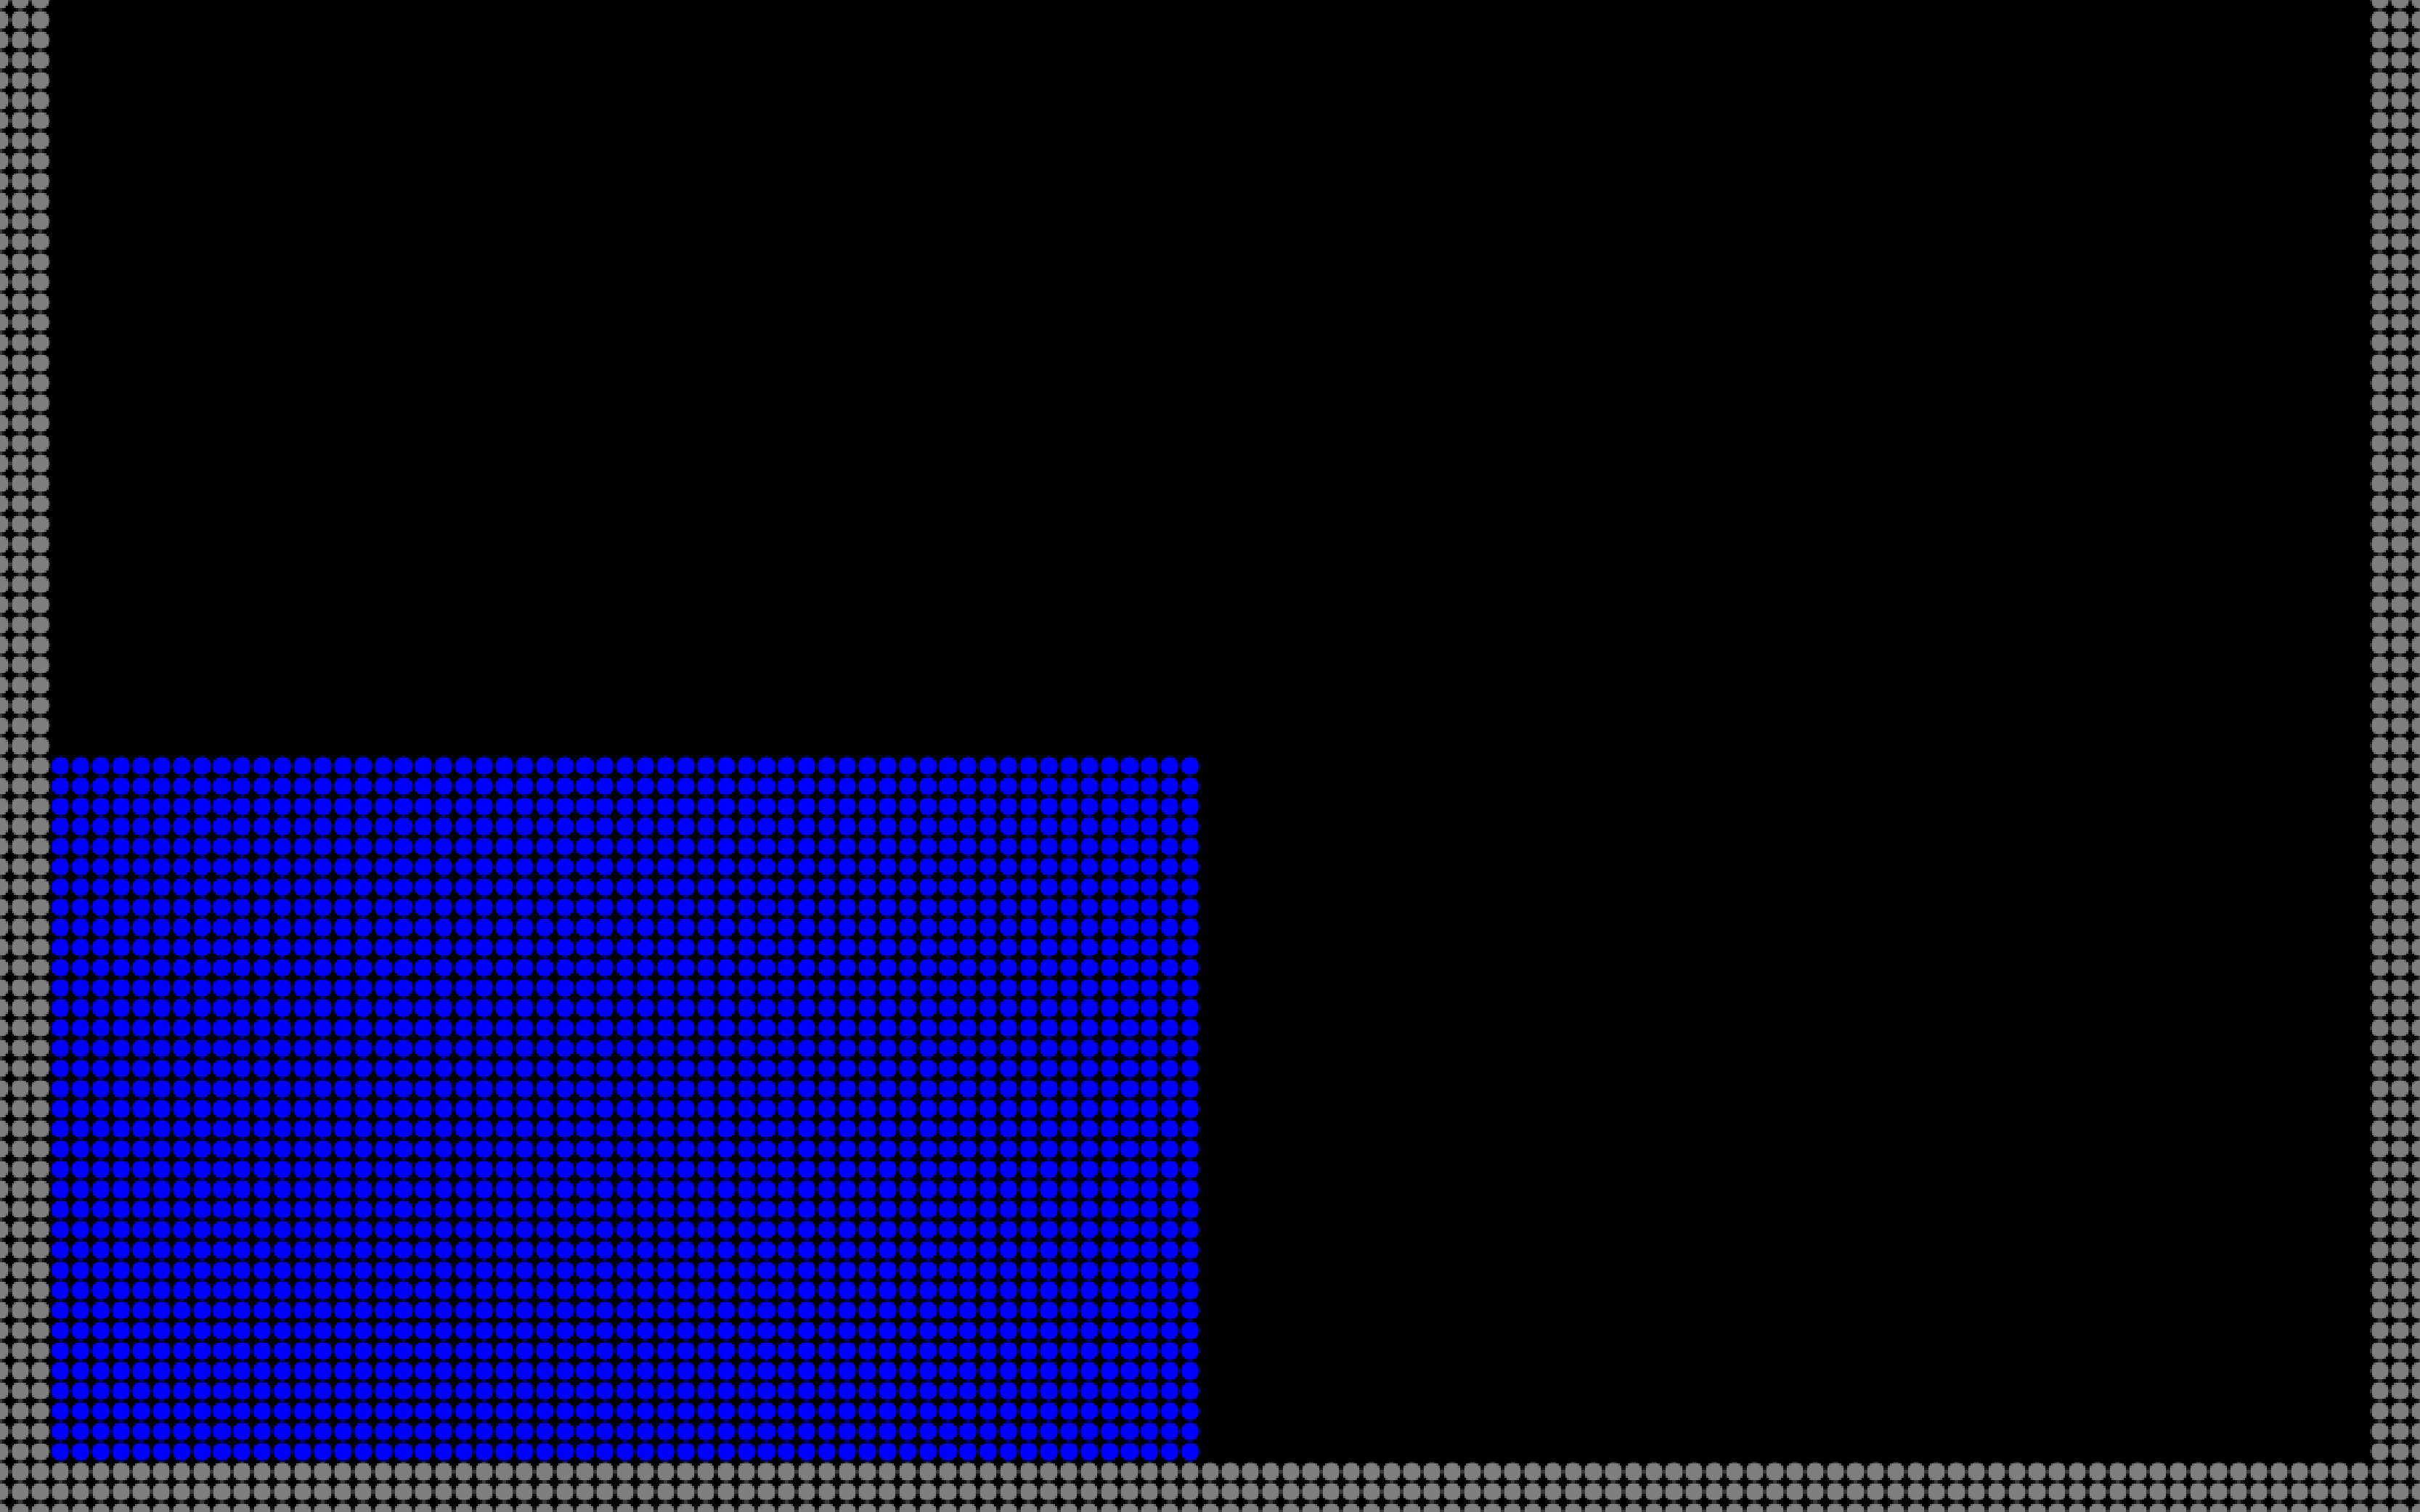
\includegraphics[width=\textwidth]{Dammbruch.png}
    \caption{Brechender Damm}
    \label{image:breaking_dam}
\end{figure}

Das zweite Szenario ist sehr ähnlich zum Dammbruchszenario. Hier ist der Damm noch vorhanden. Dieser besitzt jedoch ein Loch, wodurch die Flüssigkeit durchfließt.
In diesem Szenario kann beobachtet werden, wie die Flüssigkeit durch das Loch durchströmt und sich die Pegelstände vor und hinter dem Damm angleichen.
Der Aufbau dieses Szenarios ist in Abbildung \ref{image:leaking_dam} dargestellt.
\begin{figure}[htb]
    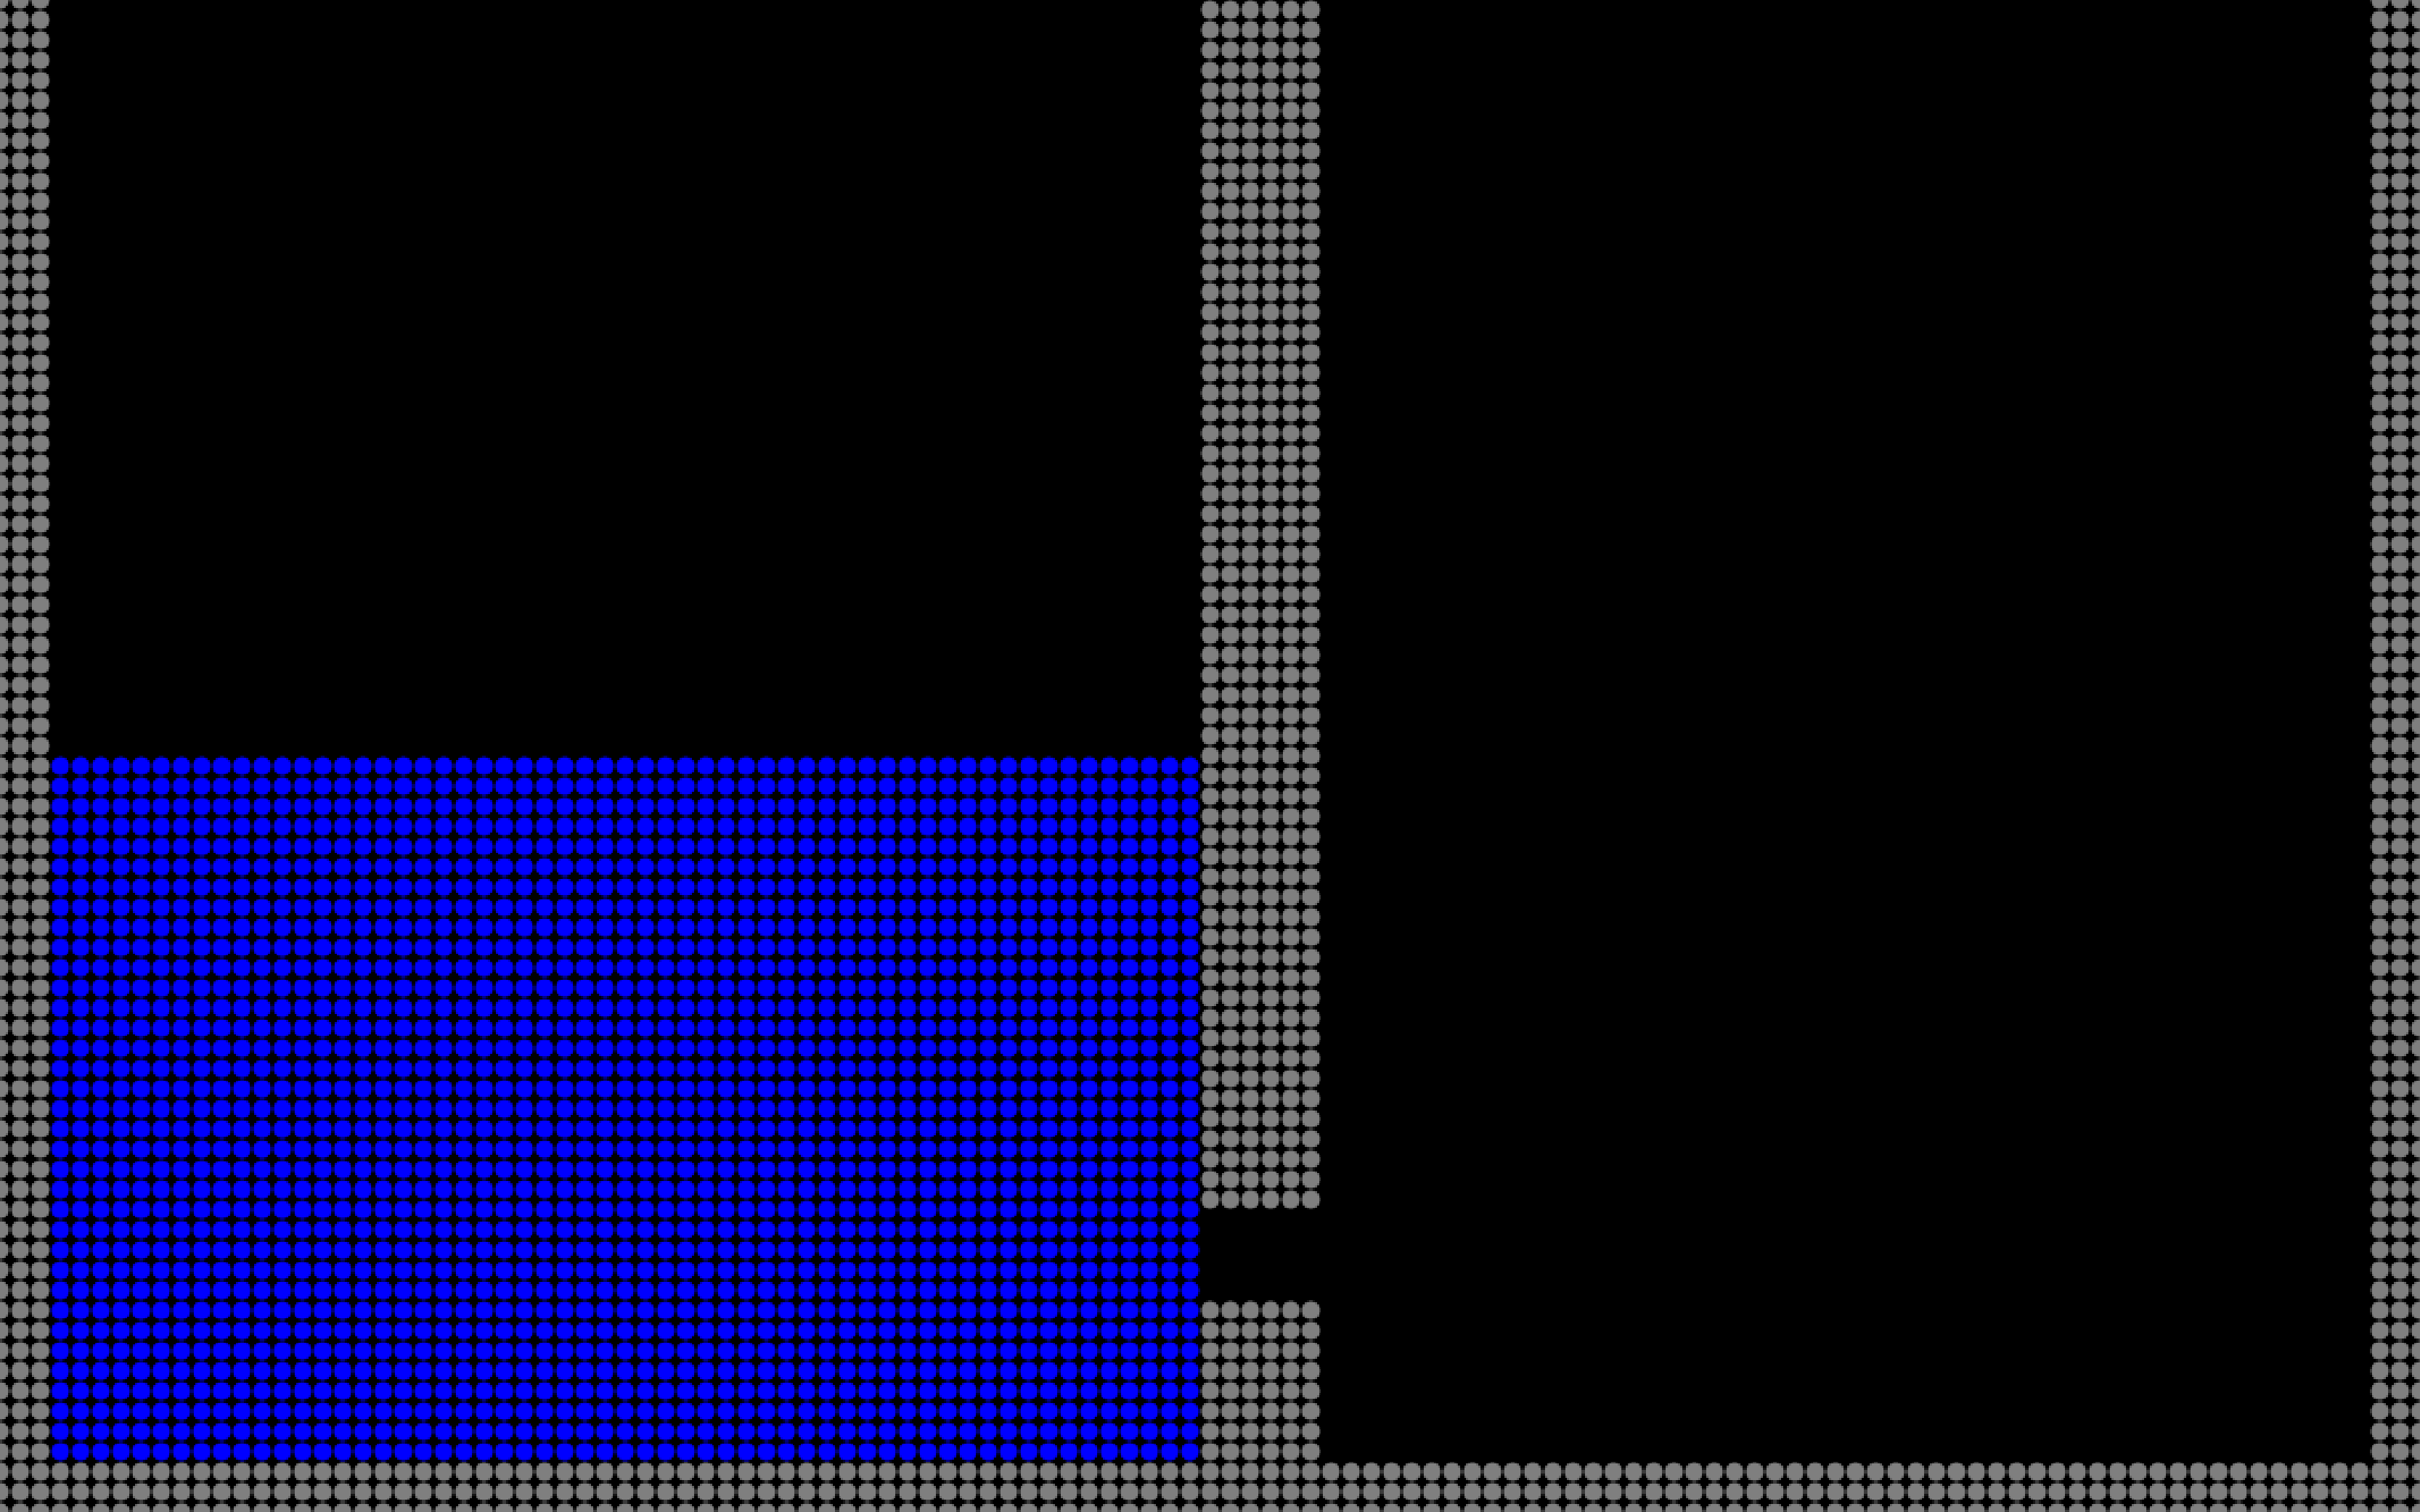
\includegraphics[width=\textwidth]{Dammleck.png}
    \caption{Damm mit Leck}
    \label{image:leaking_dam}
\end{figure}

Das dritte Szenario zeigt zu Beginn die Flüssigkeit auf einer Erhöhung.
Hier kann beobachtet werden, wie die Flüssigkeit auf beiden Seiten herunterfällt und sich zwei voneinander getrennte Flüssigkeiten bilden.
Der Aufbau dieses Szenarios ist in Abbildung \ref{image:falling_fluid} dargestellt.
\begin{figure}[htb]
    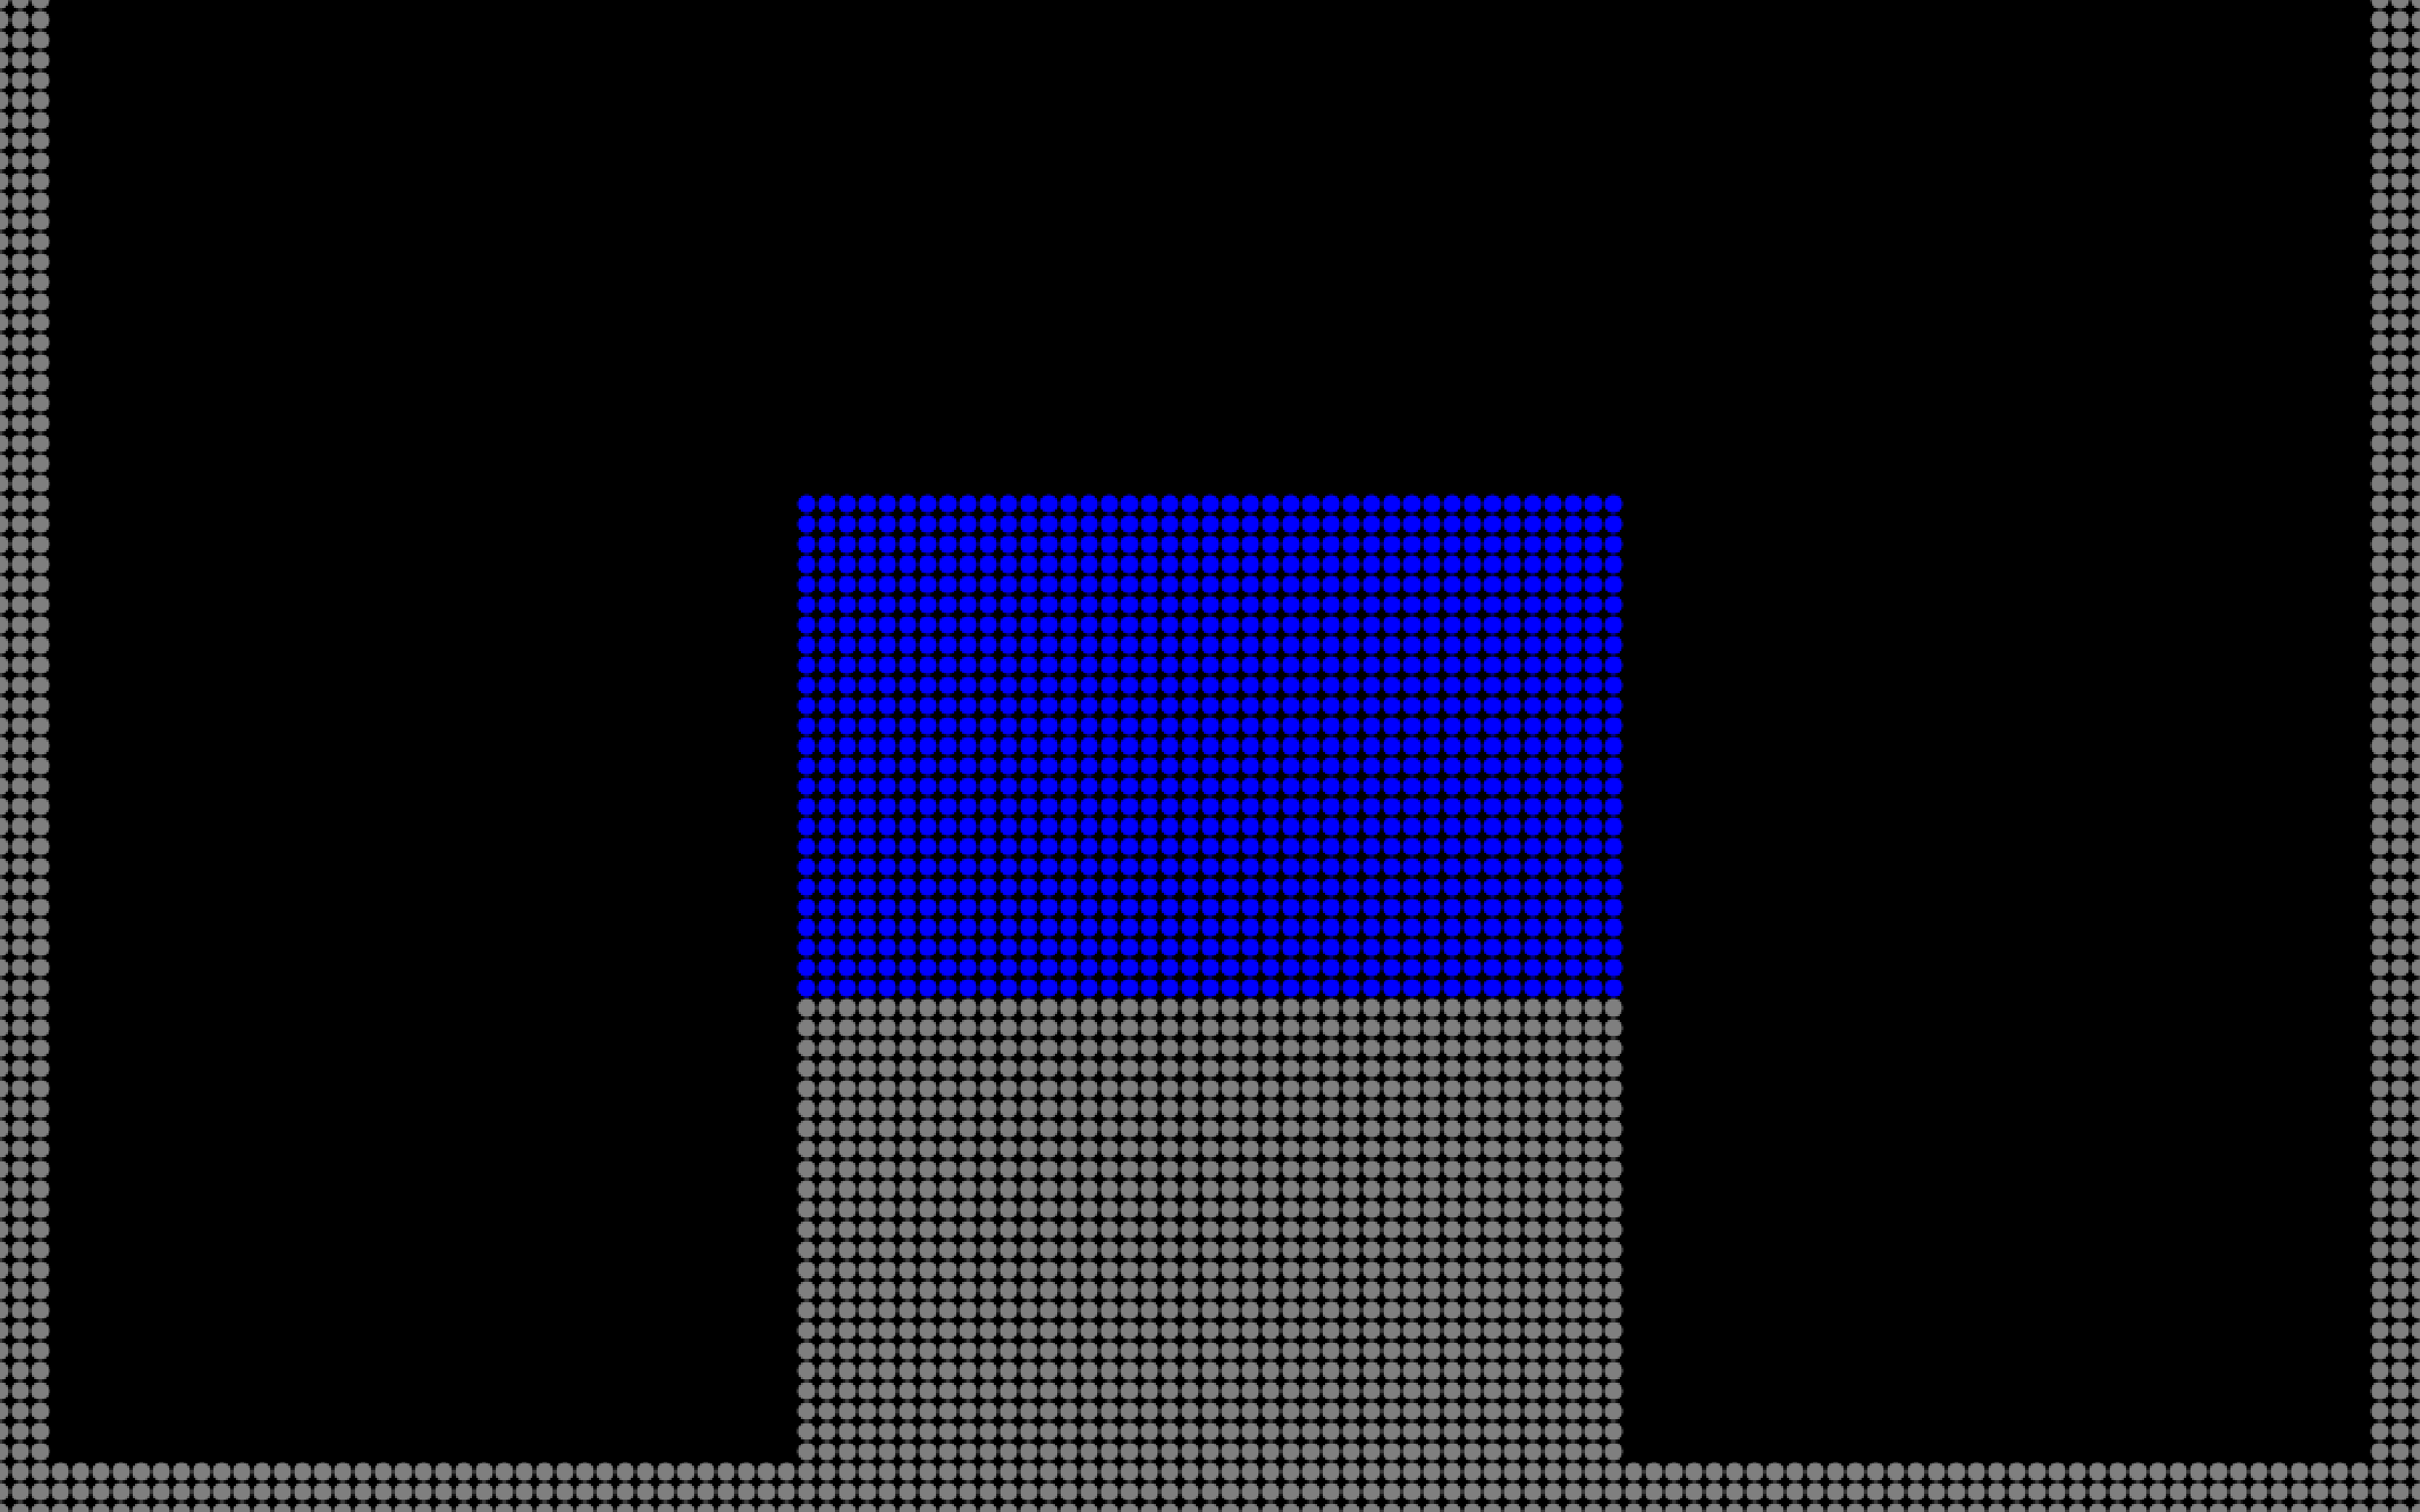
\includegraphics[width=\textwidth]{Fallend.png}
    \caption{Von einer Plattform herunterfallende Flüssigkeit}
    \label{image:falling_fluid}
\end{figure}

Im vierten Szenario kann beobachtet werden, wie die Flüssigkeit von einer schiefen Ebene in Richtung einer horizontale Ebene herunterfließt.
Dargestellt ist der Aufbau dieses Szenarios in Abbildung \ref{image:flowing_fluid}.
\begin{figure}[htb]
    \includegraphics[width=\textwidth]{Herunterfließend.png}
    \caption{Von einer schiefen Ebene herunterfließende Flüssigkeit}
    \label{image:flowing_fluid}
\end{figure}

Das fünfte Szenario zeigt eine ruhende Flüssigkeit.
Beobachtet werden kann hier wie sich die Partikel anordnen.
Dieses Szenario eignet sich auch gut, um den Verlauf der Durchschnittsdichte der Flüssigkeitspartikel zu beobachten.
Dargestellt ist der Aufbau dieses Szenarios in Abbildung \ref{image:resting_fluid}.
\begin{figure}[htb]
    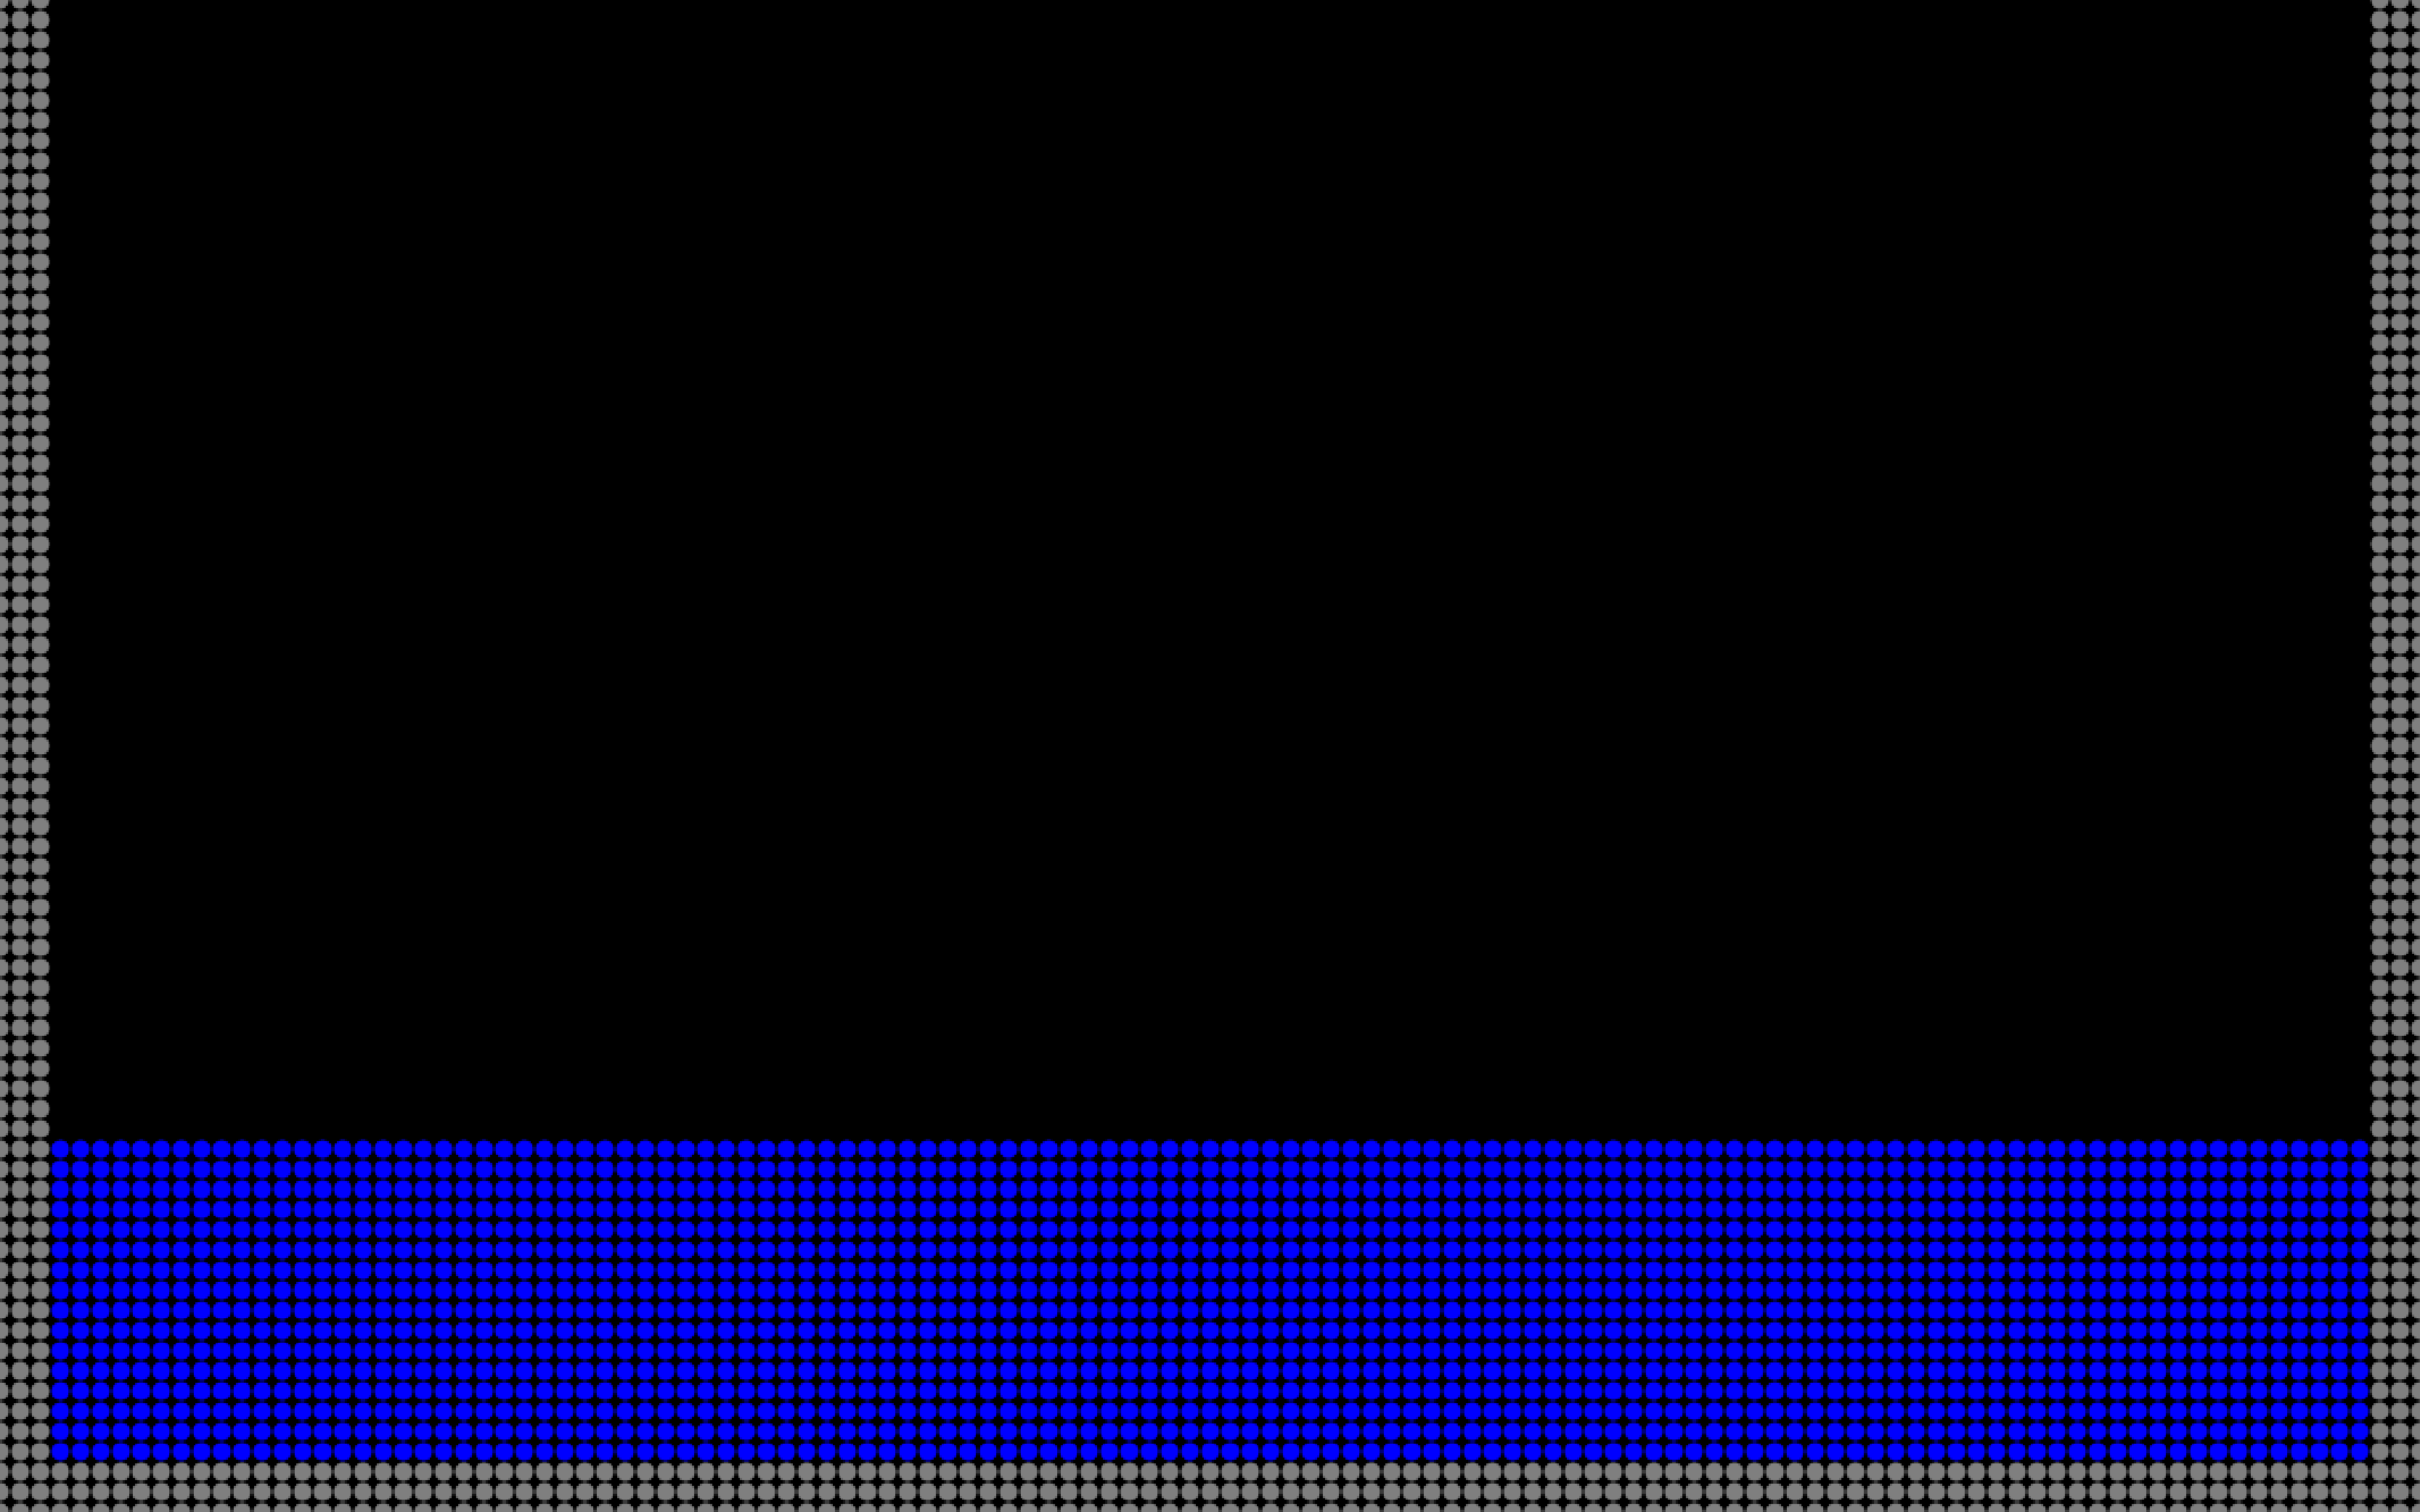
\includegraphics[width=\textwidth]{Ruhend.png}
    \caption{Ruhende Flüssigkeit}
    \label{image:resting_fluid}
\end{figure}


\section{Einfluss des Zeitschritts}
$\nu = 200$
SSPH: $k = 10^5$
\begin{figure}[htb]
    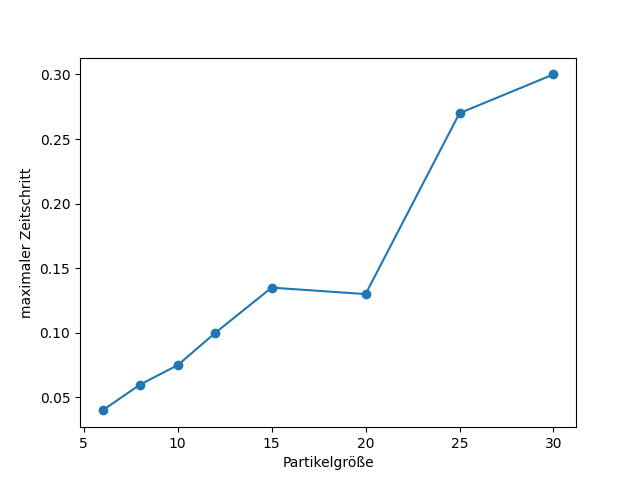
\includegraphics[width=0.8\textwidth]{particle_size_timestep_iisph.png}
    \caption{IISPH maximaler Zeitschritt nach Partikelgröße}
    \label{image:particle_size_timestep_iisph}
\end{figure}

\begin{figure}[htb]
    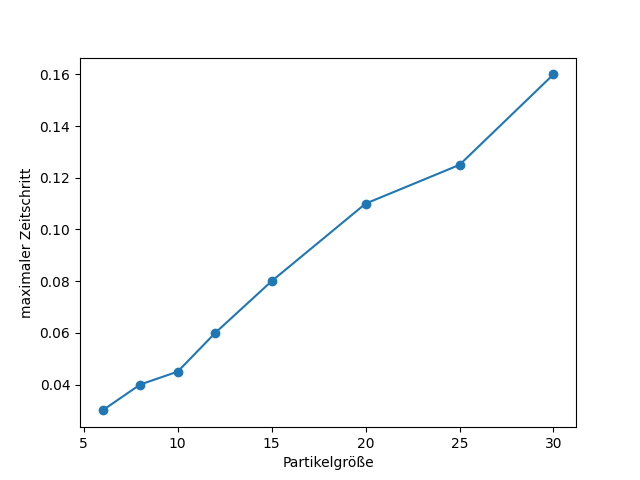
\includegraphics[width=0.8\textwidth]{particle_size_timestep_ssph.png}
    \caption{SSPH maximaler Zeitschritt nach Partikelgröße}
    \label{image:particle_size_timestep_ssph}
\end{figure}


$h = 10$
$\nu = 200$
IISPH: $\Delta t \leq 0.075$

\begin{figure}[htb]
    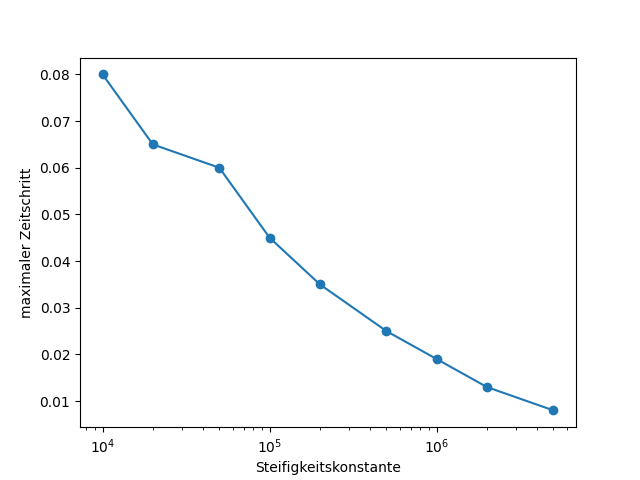
\includegraphics[width=0.8\textwidth]{stiffness_timestep_ssph.png}
    \caption{SSPH maximaler Zeitschritt nach Steifigkeitskonstante}
    \label{image:stiffness_timestep_ssph}
\end{figure}

%$h = 6, \nu = 200$, $\Delta t = 0.04$\\
%$h = 8, \nu = 200$, $\Delta t = 0.06$\\
%$h = 10, \nu = 200$, $\Delta t = 0.075$\\
%$h = 12, \nu = 200$, $\Delta t = 0.1$\\
%$h = 15, \nu = 200$, $\Delta t = 0.135$\\
%$h = 20, \nu = 200$, $\Delta t = 0.13$\\
%$h = 25, \nu = 200$, $\Delta t = 0.27$\\
%$h = 30, \nu = 200$, $\Delta t = 0.3$\\

\section{Entwicklung der Durchschnittsdichte}
Interessant ist es auch, sich die Entwicklung der Durchschnittsdichte der Flüssigkeitspartikel unterschiedlicher Simulationen anzuschauen.
Wünschenswert sind geringe Oszillationen der Durchschnittsdichte und ein Wert nahe $\rho^0$.

Dazu wurden Daten aus drei SSPH-Simulationen und einer IISPH-Simulation des Szenarios, in der die Flüssigkeit ruht, gesammelt.
Dieses Szenario wurde gewählt, weil sich hier die Partikel lediglich neu anordnen und keine großen Dichteschwankungen durch die Bewegung der Flüssigkeit zu erwarten sind.
Die Simulationen wurden durchgeführt an Partikel mit Größe $h=10$ und Viskosität $\nu = 200$.
Für die IISPH-Simulation wurde ein Zeitschritt $\Delta t = 0.1$ gewählt.
Damit wurden 1000 Simulationsschritte ausgewertet.

In den SSPH-Simulationen wurden drei verschiedene Steifigkeitskonstanten gewählt.
Einmal ein niedriger Wert $k = 10^4$, ein mittlerer Wert $k = 10^5$ und ein hoher Wert $k = 10^6$.
Da die beiden höheren Werte für die Steifigkeitskonstante keinen Zeitschritt $\Delta t = 0.1$ erlauben, wurden hier niedrigere Zeitschritte von $\Delta t = 0.05$
und $\Delta t = 0.01$ gewählt.
Um jedoch die Entwicklung der Durchschnittsdichte mit der IISPH-Simulation zu vergleichen und die gleiche Zeitspanne zu beobachten,
wurde hier eine größere Anzahl an Iterationen von 2000 Iterationen bzw. 10000 Iterationen festgelegt.

Das Diagramm in Abbildung \ref{image:average_density_iisph} zeigt die Entwicklung der Durchschnitte in der IISPH-Simulation nach Iteration.
%$h = 10, \nu = 200$, $\Delta t = 0.1$\\
%$h = 10, \nu = 200$, $\Delta t = 0.1, k = 10^4$\\
%$h = 10, \nu = 200$, $\Delta t = 0.05, k = 10^5$\\
%$h = 10, \nu = 200$, $\Delta t = 0.01, k = 10^6$

\begin{figure}[htb]
    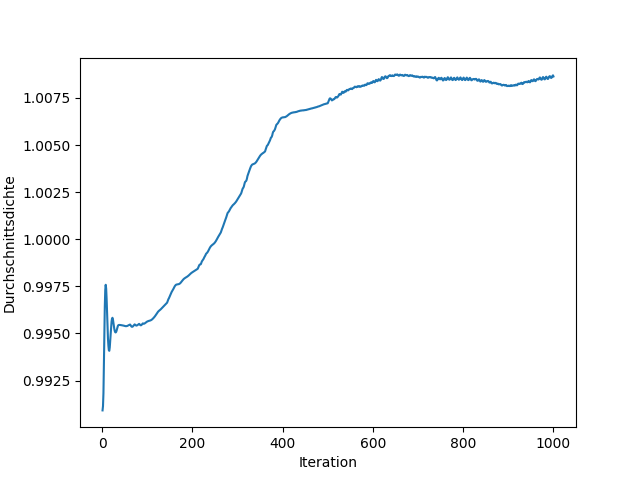
\includegraphics[width=0.8\textwidth]{average_density_iisph.png}
    \caption{IISPH Durchschnittsdichte}
    \label{image:average_density_iisph}
\end{figure}

Die Diagramme aus den Abbildungen \ref{image:average_density_ssph_low_stiffness}, \ref{image:average_density_ssph_mid_stiffness}, \ref{image:average_density_ssph_high_stiffness}
zeigen die Entwicklung der Durchschnitte in den SSPH-Simulationen nach Iteration.

\begin{figure}[htb]
    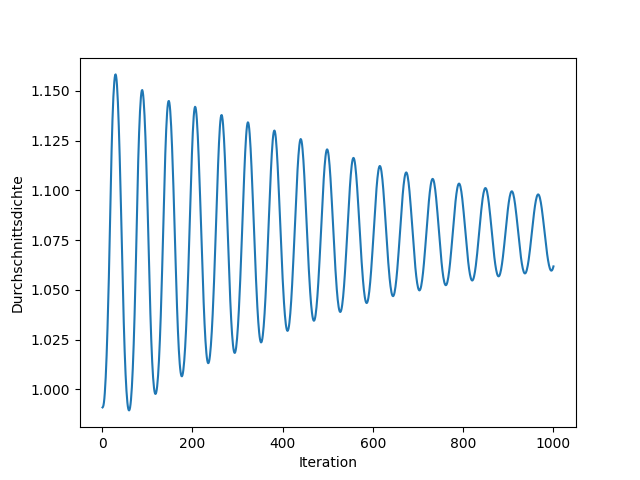
\includegraphics[width=0.8\textwidth]{average_density_ssph_low_stiffness.png}
    \caption{SSPH Durchschnittsdichte mit niedriger Steifigkeitskonstante}
    \label{image:average_density_ssph_low_stiffness}
\end{figure}

\begin{figure}[htb]
    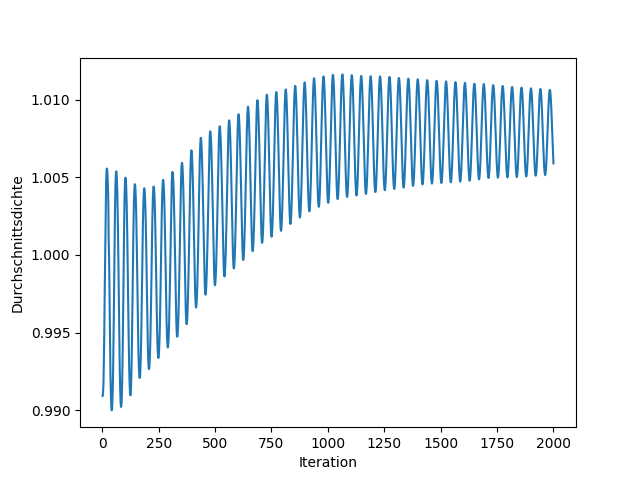
\includegraphics[width=0.8\textwidth]{average_density_ssph_mid_stiffness.png}
    \caption{SSPH Durchschnittsdichte mit mittlerer Steifigkeitskonstante}
    \label{image:average_density_ssph_mid_stiffness}
\end{figure}

\begin{figure}[htb]
    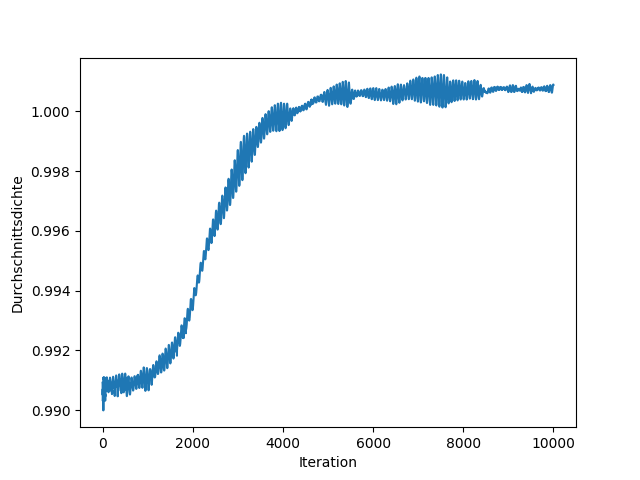
\includegraphics[width=0.8\textwidth]{average_density_ssph_high_stiffness.png}
    \caption{SSPH Durchschnittsdichte mit hoher Steifigkeitskonstante}
    \label{image:average_density_ssph_high_stiffness}
\end{figure}

In den Diagrammen ist zu erkennen, dass sich bei SSPH mit zunehmender Steifigkeitskonstante die Oszillationen abschwächen.
Mit einer Steifigkeitskonstante von $k = 10^4$ dominieren die Oszillationen die Entwicklung der Durchschnittsdichte,
während bei einer Steifigkeitskonstante von $k = 10^6$ die Durchschnittsdichte deutlich weniger oszilliert.
In allen Simulationen ist zu sehen, dass mit der Zeit die Amplituden der Oszillationen geringer werden.
In IISPH sind die Oszillationen kaum zu erkennen.
Dadurch, dass für die gleiche Zeitspanne zehn mal weniger Iterationen berechnet werden müssen und zudem die Oszillationen sehr schwach sind,
ist IISPH hier im Vorteil.


\section{Rechenaufwand}
Wichtig zu berücksichtigen ist ebenfalls, den Rechenaufwand der unterschiedlichen Druckberechnungsmethoden anzuschauen.
Dazu wurden Daten aus acht Dammbruchsimulationen gesammelt, davon sechs mit IISPH und zwei mit SSPH.
Die Partikelgröße $h$ beträgt dabei jeweils 10 und die Viskosität $\nu$ ist jeweils auf 200 festgelegt.
Der Zeitschritt $\Delta t$ und die Steifigkeitskonstante $k$ in SSPH variieren nach Simulation.

Ermittelt wurde die benötigte Zeit für 100 Simulationsschritte.
Daraus wurde die durchschnittliche Zeit $\overline{t}_{step}$ für einen Simulationsschritt berechnet.
Setzt man diesen Wert in Verhältnis zum Zeitschritt $\Delta t$, so erhält man einen Anhaltspunkt, wie schnell sich äquivalente Sequenzen der Simulation berechnen lassen.
Sollte die Simulation möglichst schnell berechnet werden, so ist ein möglichst geringer Wert für das Verhältnis $\overline{t}_{step} / \Delta t$ wünschenswert.

Die Simulationen wurden auf dem Prozessor \textit{Intel® Core™ i5-6600k} berechnet, welcher 4 Kerne besitzt und auf eine Taktfrequenz von 4 Ghz übertaktet ist.

\begin{center}
    \begin{tabular}{ r r r | c c }
        & & & $\overline{t}_{step}$ & $\overline{t}_{step} / \Delta t$\\
        SSPH & $\Delta t = 0.01$ & $k = 10^6$ & 53 ms & 5300\\
        SSPH & $\Delta t = 0.05$ & $k = 10^5$ & 53 ms & 1060\\
        %SSPH & $\Delta t = 0.1$ & $k = 10^4$ & 55 ms & 550\\
        IISPH & $\Delta t = 0.01$ & & 128 ms & 12800\\
        IISPH & $\Delta t = 0.02$ & & 127 ms & 6350\\
        IISPH & $\Delta t = 0.03$ & & 145 ms & 4833\\
        IISPH & $\Delta t = 0.05$ & & 164 ms & 3280\\
        IISPH & $\Delta t = 0.08$ & & 191 ms & 2388\\
        IISPH & $\Delta t = 0.1$ & & 210 ms & 2100\\
    \end{tabular}
\end{center}

Aus diesen Daten lässt sich erkennen,
dass in IISPH für einen größeren Zeitschritt $\Delta t$ die durchschnittliche Berechnungszeit $\overline{t}_{step}$ pro Simulationsschritt zunimmt.
Jedoch sinkt das Verhältnis $\overline{t}_{step} / \Delta t$ gleichzeitig, weswegen die Berechnung durch größere Zeitschritte insgesamt effizienter ist.

In SSPH ist $\overline{t}_{step}$ relativ konstant, weil bei der Druckberechnung kein Gleichungssystem iterativ gelöst werden muss,
wo durch größere Zeitschritte auch größere Fehler entstehen, was die Druckberechnung verlängert.
In SSPH kann jedoch für die Steifigkeitskonstante $k = 10^6$ nur maximal ein Zeitschritt von $\Delta t = 0.01$ gewählt werden,
da die Simulation für größere Zeitschritte sonst instabil wird.
Um in SSPH größere Zeitschritte wählen zu können,  muss eine geringere Steifigkeitskonstante gewählt werden, was jedoch zu einer weniger realistischen Simulation führt.

\chapter{Fazit und Ausblick}
\bibliographystyle{alpha}
\bibliography{literaturverzeichnis}


\end{document}
